\documentclass[12pt]{article}
\usepackage{amsmath}
\usepackage{amssymb}
\usepackage{graphicx}
\usepackage{float}
\usepackage{listings}
\usepackage{xcolor}
\usepackage[parfill]{parskip}
\usepackage{caption}
\usepackage{subcaption}
\setlength{\oddsidemargin}{0in}
\setlength{\evensidemargin}{0in}
\setlength{\textheight}{9in}
\setlength{\textwidth}{6.5in}
\setlength{\topmargin}{-0.5in}
 
\definecolor{codegreen}{rgb}{0,0.6,0}
\definecolor{codegray}{rgb}{0.5,0.5,0.5}
\definecolor{codepurple}{rgb}{0.58,0,0.82}
\definecolor{backcolour}{rgb}{0.95,0.95,0.92}
\lstdefinestyle{mystyle}{
    backgroundcolor=\color{backcolour},   
    commentstyle=\color{codegreen},
    keywordstyle=\color{magenta},
    numberstyle=\tiny\color{codegray},
    stringstyle=\color{codepurple},
    basicstyle=\ttfamily\footnotesize,
    breakatwhitespace=false,         
    breaklines=true,                 
    captionpos=b,                    
    keepspaces=true,                 
    numbers=left,                    
    numbersep=5pt,                  
    showspaces=false,                
    showstringspaces=false,
    showtabs=false,                  
    tabsize=2
}
\lstset{style=mystyle}
%%%%%%%%%%%%%%%%%%%%%%%%%%%%%%%%%%%%%%%%%%%%%%%%%%%%%%%%%%%%%%%%%%%%%%%%%%%
\title{\bf Term Project\\[2ex] 
       \rm\normalsize ECS 132 --- Fall 2019}
\date{\today}
\author{\bf Vincent Boc, Derek Li, Nikhil Razdan}

\begin{document}
\maketitle


%%%%%%%%%%%%%%%%%%%%%%%%%%%%%%%%%%%%%%%%%%%%%%%%%%%%%%%%

\tableofcontents
\newpage

\section{Part A}

\subsection{Vincent Boc's Poster}
\begin{figure}
	\centering
  	
\includegraphics[width=150mm]{poster0.jpg}
 	\caption{Poster in Question}
 	\label{fig:vincent_poster}
\end{figure}

\subsubsection{Professor's Credentials}
The professor that was involved in this is Dr. Michael Springborn, P.H.D Department of Environmental Science and Policy.

\subsubsection*{Poster's Topic}
This poster seeks to establish whether or not there is a correlation between the decline of amphibians in (1980-1995) and human malaria cases.. In other words, the poster analyzes whether or not there is a relationship between human diseases and the declining population of amphibians. 

\subsubsection{Poster's Method}
In order to analyze whether or not there is a correlation, the poster utilized a log-linear regression model with malaria cases against declining population of amphibians. In doing so, it concluded that there is a significant negative correlation with $p < 0.01$.

\subsubsection{Improving through Confidence Intervals} 
In order to understand why confidence intervals, it is best to note what the p-value is testing here. The p-value is testing the null hypothesis that the coefficient for the regression model is 0, or in other words there is no correlation. Therefore with a $p < 0.01$, it states that assuming the null hypothesis is true, we will only see a negative correlation 0.01\% of the time.

However, this is not a good method of testing correlation, as it does not tell as much information as confidence intervals do. A 95\% confidence interval for log-linear regression model will include the range that the true correlation efficient will lie in 95\% of the time conducting this observation. In other words, it gives us a range in which the true correlation coefficient lies in for 95 out of 100 repetitions.

This information of having the range that contains the true correlation coefficient is a lot more useful than the information that p-value gives which is just a probability that there is a negative correlation assuming the null hypothesis is true.

\newpage
\subsection{Nikhil Razdan's Poster}
\begin{figure}
	\centering
  	
\includegraphics[width=150mm]{nikhil_poster.jpg}
 	\caption{Poster in Question}
 	\label{fig:Nikhil_poster}
\end{figure}

\subsubsection{Overview}
This poster, sponsored by Dr. Rebecca Calisi Ph.D. and Suzanne Austin Ph.D., focuses on the relationship between socially dominant parents and the quality of their offspring. Their subjects are a number of pigeons at the Calisi Lab.

\subsubsection{Methodology}
There are two main scientific hurdles to overcome to complete the experiment: measuring the parent's social dominion and the children's quality. These are inherently hard things to measure, but the researchers developed their own methods.

To measure the social dominance of the parents, the researchers recorded 5 hours of footage of the birds and noted every time they expressed dominant behavior, including chasing and pecking other birds. They then converted these observations into a score of dominance, which they term an Frequency Success Index (FSI).

To calculate the quality of the offspring, they combined measurements of the tarsus length to mass ratio at 25 days old and the quality of the its incubation.

\subsubsection{P-value} 
The p-value of an experiment measures the probability of achieving the measured output assuming that the null hypothesis holds. In other words, it represents the chance that we measured our data given the null hypothesis is correct. 

It is worth noting two things. This first is that this is a conditional probability. This means that we are ignoring the cases where the null hypothesis is incorrect in our calculation. The second is that the null hypothesis is the opposite of what we're testing, which in this case represents no correlation or a negative correlation. Applying these two pieces of information, we get the intention of the p-value: to measure the probability that the null hypothesis is false, and thus our desired hypothesis is true.

We get to this because, by rejecting the null hypothesis, that means that our hypothesis is the only remaining option. Thus, a lower p-value means a higher probability of rejecting the null hypothesis, and a higher probability that we must accept the alternative hypothesis.

\subsubsection{Problems with the P-Value}
There is one major problem with the usage of a p-value: it doesn't actually prove that our hypothesis is true. Instead, it shows the probability that we could not have gotten our data with the opposite hypothesis. This is dangerous because it ignores the impact of other factors. However, we can minimize these issues by using confidence intervals instead of significance testing.

\subsubsection{Confidence Intervals}
Confidence intervals instead predict the range in which the actual coefficient of our model lies. This means that it will actually predict our degree of correlation. Unlike with a p-value, this will give an estimate of the quality of our model, rather than an estimate of the chance our model is incorrect.

For example, a 99\% confidence interval in this example would mean that there is a 99\% chance that the true coefficient of our model is within the tested range. Hence, in every 100 trials, we can expect 1 to have a coefficient outside that calculated range.

\newpage
\subsection{Derek Li's Poster}
\begin{figure}
	\centering
  	
\includegraphics[width=150mm]{poster1.jpg}
 	\caption{Poster in Question}
 	\label{fig:derek_poster}
\end{figure}
\subsubsection{Introduction}
In the UC Davis Academic Posters Gallery, I chose the poster titled, “Prey preference and growth of juvenile sea star Pisaster ochraceus.” The UCDavis professor involved in this research is Eric Sanford, Ph. D., College of Biological Sciences, Evolution and Ecology. The goal of this research was to find out the prey preference of Pisaster ochraceus, and their growth when given a certain diet, among snails, mussels, and barnacles. With six different diets, each consisting of one or more of the possible prey, five trials were completed for each one. The results were mainly based on the total biomass of prey eaten.
\subsubsection{Usage of P-values}	
With a p-value of 0.0001, the research concluded that there is strong evidence of Pisaster ochraceus growing the most when eating mussels. In addition, with p-values of 0.065 and 0.052, the research concluded that the Pisaster ochraceus preferred mussels over snails and barnacles, respectively. However, simply relying on p-values can be dangerous and misleading, especially when the research seems to be using it to justify the correctness of its hypothesis, which stated that barnacles would be the most preferred prey. Using the p-value of 0.0001, the research stated that its data showed a statistically significant difference because the mussels were actually the most preferred prey by a big margin. By only relying on the p-values, it seems that the research concluded that the hypothesis was incorrect. With just a sample size of 5 trials for each diet, one can argue that this data does not provide an actual, true representation of what the Pisaster ochraceus prefers. This brings up the question, “If we repeat this experiment multiple times, would we relatively come to the same conclusion?” Due to this small sample size, the usage of confidence intervals would provide a more insightful analysis on this research. With confidence intervals, the research would be able to provide a more compelling argument about its results.

\newpage
\section{Part B}
\subsection{Disclaimer: ATemp} \label{disclaimer}
In day1's dataset, ATemp most likely stands for actual temperature, but we opted to call it Atmospheric temperature. This is due to the fact that our graphs compare predicted temperature vs actual temperature, where actual temperature is referring to the "real" value of the temperature from the dataset. Or in other words, when we speak of actual temperature, we are referring to day1\$temp. When we speak of atmospheric temperature, we are referring to day1\$atemp.

\subsection{The Goal} \label{goal}
The goal for this problem is to predict all of the weather variables for a day based on the past days. In order to do this, we opted to create models for all of the individual weather variables.

\subsection{The Criteria for a Good Model} \label{criteria}
The criteria is as follows:
\begin{enumerate}
	\item Low k value (Recentness) 
	\item High R-squared value (without overfitting)
	\item Prediction Accuracy
\end{enumerate}
	
\subsection{Predicting Temperature} \label{predictingtemp}
\subsubsection{What Influences Temperature?} \label{temp_params}
In order to predict temperature, we must analyze some possible factors of temperature. To do this, I first plotted the graph of Temperature vs. Days for all 731 days provided in the data set.
\begin{figure}[H]
	\centering
  	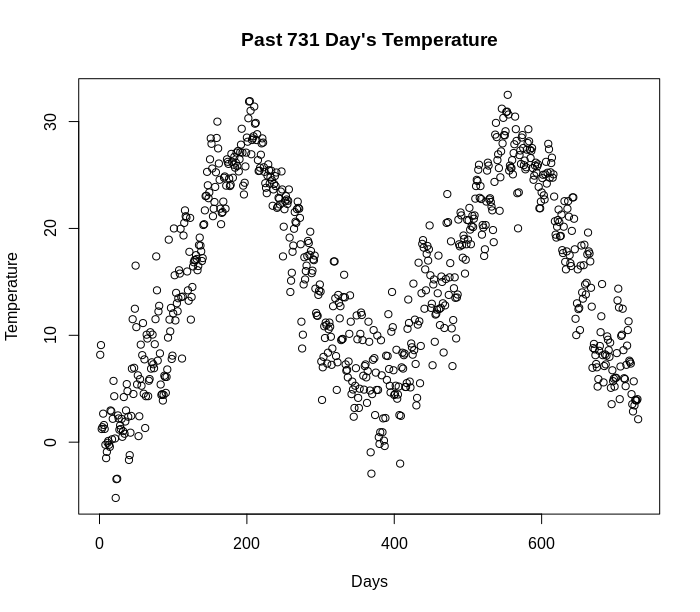
\includegraphics[width=100mm]{dayvstemp.png}
 	\caption{Day vs. Temp}
 	\label{fig:dayvstemp}
\end{figure}

From this graph, it becomes apparent that the temperature of the past 731 days fluctuates up and down resembling a "M" curve. In other words, it seems cyclic similar to a sin curve. This leads me to believe that one of the parameters of the model is cyclic, or seasonal. Thus, I have the hypothesis that season plays a role in determining temperature.

In order to find out whether or not season plays a large role in determining temperature, I plotted the graph of season vs temperature and looked at the median and mean values.
\begin{figure}[H]
	\centering
  	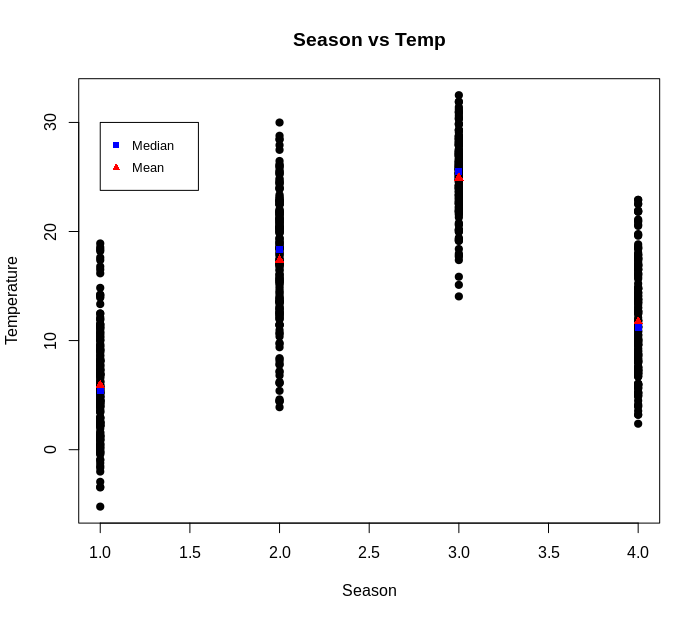
\includegraphics[width=150mm]{seasonvstemp.png}
 	\caption{Season vs. Temp}
 	\label{fig:seasonvstemp}
\end{figure}
This graph displays a clear trend that winter (season number 1), obviously, is on average the coldest season. Following that, the seasons gradually warm up until it hits summer (season number 3) until it cools back down in the fall (season number 4). It also becomes apparent from this, that this is similar to the "M" shape that was found in \ref{fig:dayvstemp}.

This further reaffirms my hypothesis that season will play an integral role in predicting the temperature. Additionally, we can find out the correlation value between temperature and season by executing the following:
\begin{verbatim}
> cor(day1$temp, day1$season)
[1] 0.3343149
\end{verbatim}
Since the correlation value is 0.33, there is a moderate correlation between the two and should be taken into account.

Additionally, the temperature from the previous days should play a role in predicting the temperature. For example, if the temperature the couple of days before is low, then the temperature for the current day would be on the lower end as well. The same would apply if the temperatures the past couple of days are on the higher end, then the current day's temperature would be on the higher end. Therefore, past temperatures would play an integral role.

Similarly, the atmospheric temperature would play a role too. This is due to the fact that atmospheric temperature has a relationship with temperature. Therefore, if the temperature from the previous days are colder, the atmospheric temperature would be colder for the most part, excluding extreme humidity and wind speed (more on this in the predicting weather conditions section).

This can be confirmed by examining the correlation again:
\begin{verbatim}
> cor(day1$temp, day1$atemp)
[1] 0.9917016
\end{verbatim}
This implies a very strong correlation.

However, the other weather variables such as humidity, wind speed, or weather conditions should not influence temperature or rather have a noticeable impact on them. For humidity or wind speed, those do not have a large impact on the raw value of temperature, but rather they have an impact the feeling temperature, or which we shall call atmospheric temperature. 

As for weather conditions, they do have an impact on temperature as clouds are able to trap heat in or block heat out. However, this was chosen to be excluded in fear of over-fitting and the fact that weather conditions are somewhat unreliable in predictions. These two disadvantages make including weather conditions as a parameter undesirable.

Therefore, our parameters are Past Temperature, Past Atmospheric Temperature (atemp), and the Seasons.

\subsubsection{Building the Model for Temperature}
For this model, I chose to use linear modeling rather than KNN on the premise that it allowed me to monitor any changes I made to the predictor variables polynomial-wise. The formula will be very simple, but we have to create 3 dummy variables for the winter, spring, and summer. Fall will be when all 3 dummy variables are equal to zero.

Since my parameters rely on weather variables from past days, I had to define a variable k, which will dictate how many days back our model would look at. This comes with the trouble of finding out what the most optimal value of k would be.

\subsubsection{Finding the Optimal Value of k} \label{finding}
The most optimal value of k can be determined through trial and error and careful analysis of the linear model. My first instinct was to start with a low k value of 2 and then increase it until I notice a decrease in performance.

However, this method uses a lot of repeatable steps which are:
\begin{enumerate}
  \item Build the training data set for k values and the parameters listed in \ref{temp_params}.
  \item Running linear modeling for the training data set.
  \item Calculate all the predicted values for days outside the training set.
  \item Graph the predicted values against actual temperature for days outside of the training data set's range.
\end{enumerate}

Since our goal is cross-validation, we want to select a specific subset of days from our data to use as the training and the rest to cross-validate. I chose to include a whole year in the training set because it would allow the model to train on all of the seasons and have many reliable samples rather than random samples.

Thus, I created a series of functions that are easily callable that do the listed steps. Step 1 would be createDataTrainingTemp(), 2 would be runLMTempTemp(), and three would be crossValidateTemp().

Thus, doing this for $k=2$ gave the graph below:

\begin{figure}[H]
	\centering
  	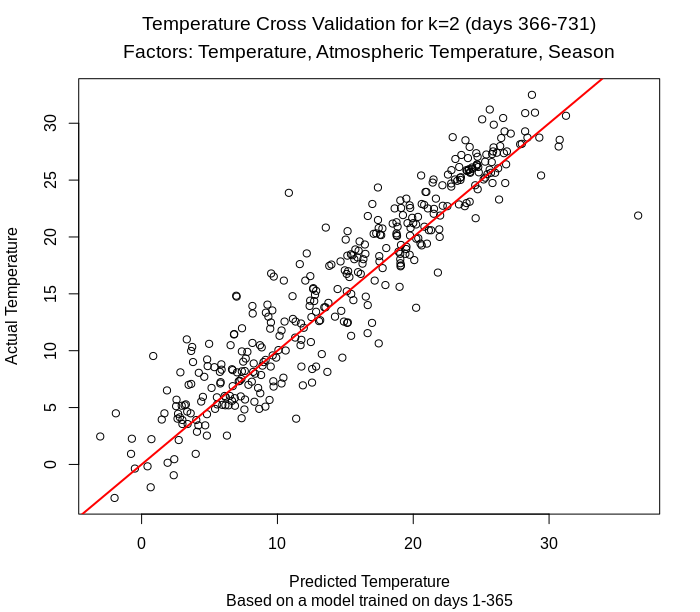
\includegraphics[width=112mm]{tempxvalidk=2.png}
 	\caption{Temperature Cross Validation for k = 2}
 	\label{fig:tmpxvalid2}
\end{figure} 

To explain this graph, we graphed the predicted temperature for days 366-731 which is outside of our training data set. The red line represents the y=x line, which means that if a point were to land on there, the predicted temperature = the actual temperature. Therefore, the closer the points are to the line, the more accurate our model.

From this graph, we can see that our three parameters give us a relatively good fit! All of the points are slightly close to the line, but not too far where it means that our parameters are wrong. There are some outliers in the graph of course, but those can be safely ignored as there are only two noticeable outliers. Therefore, we can keep going with our three parameters and focus on optimizing our k values. 

Additionally, we can analyze the output of R's lm() function which is used to create a linear model for our predictive variables and response variable.

This is k=2's lm() output:
\begin{verbatim}
Residuals:
    Min      1Q  Median      3Q     Max 
-9.0067 -1.2958  0.1035  1.4511  7.2918 

Coefficients:
                   Estimate Std. Error t value Pr(>|t|)    
(Intercept)         1.66826    0.78070   2.137 0.033296 *  
trainingdata[, 1]   0.58618    0.20764   2.823 0.005028 ** 
trainingdata[, 2]  -0.56300    0.16118  -3.493 0.000538 ***
trainingdata[, 3]   0.09404    2.25335   0.042 0.966734    
trainingdata[, 4]   1.92441    2.59972   0.740 0.459649    
trainingdata[, 5]   0.89493    2.29386   0.390 0.696668    
trainingdata[, 6]   0.30058    0.22055   1.363 0.173789    
trainingdata[, 7]   0.52687    0.16547   3.184 0.001582 ** 
trainingdata[, 8]  -1.10347    2.24024  -0.493 0.622627    
trainingdata[, 9]  -0.88764    2.59042  -0.343 0.732058    
trainingdata[, 10]  1.21120    2.26554   0.535 0.593251    
---
Signif. codes:  0 ‘***’ 0.001 ‘**’ 0.01 ‘*’ 0.05 ‘.’ 0.1 ‘ ’ 1

Residual standard error: 2.555 on 352 degrees of freedom
Multiple R-squared:  0.9203,	Adjusted R-squared:  0.918 
F-statistic: 406.4 on 10 and 352 DF,  p-value: < 2.2e-16
\end{verbatim}

The three values that are important to look at are residuals, R-squared, and Adjusted R-squared. For k=2, we note that our residuals minimum is $-9.0067$ and max is $7.2918$. This is seems alarming, but the median residual is merely $0.1035$ which may mean that those min and max are quite possibly the outliers we saw in Figure \ref{fig:tmpxvalid2}.

Therefore, we repeat this process for k values incremented by 1 until we notice a decrease in accuracy.

Here are the results of this process (k=3, k=4, k=5, k=7):
\begin{figure}[H]
\begin{tabular}{cc}
  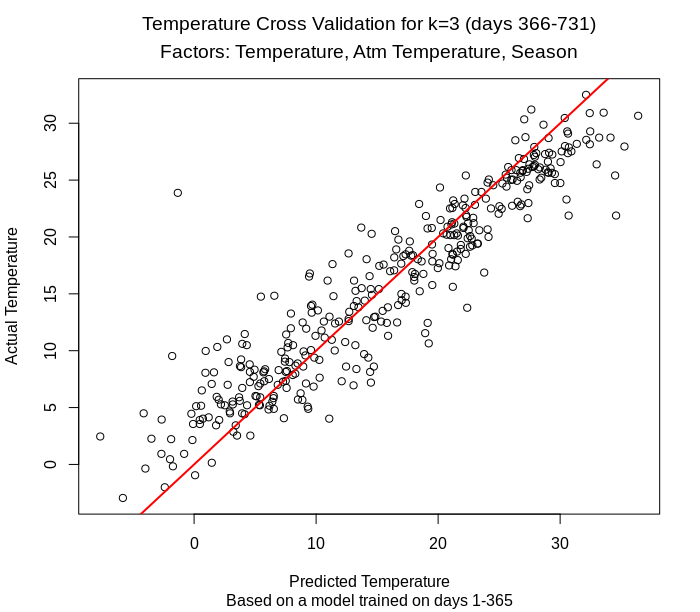
\includegraphics[width=.5\linewidth]{tempxvalidk=3.png} &   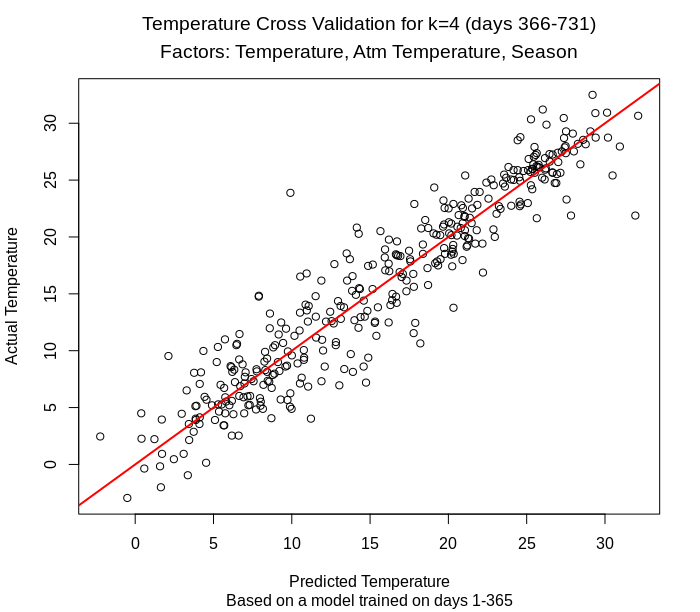
\includegraphics[width=.5\linewidth]{tempxvalidk=4.png} \\
(a) k = 3 & (b) k = 4 \\[6pt]
 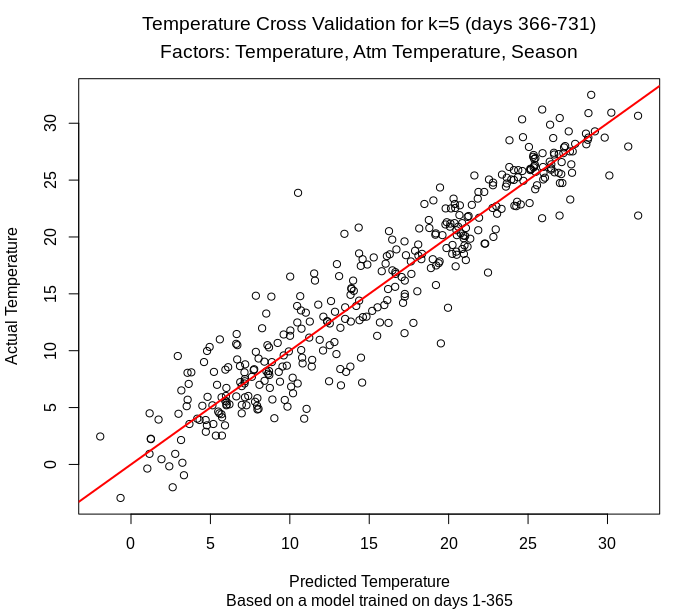
\includegraphics[width=.5\linewidth]{tempxvalidk=5.png} &   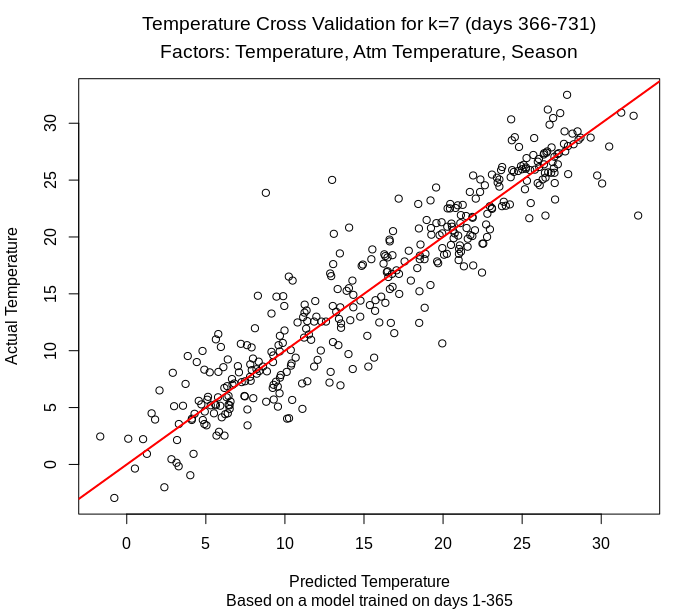
\includegraphics[width=.5\linewidth]{tempxvalidk=7.png} \\
(c) k = 5 & (d) k = 7 \\[6pt]
\end{tabular}
\caption{Result of Repeating the Process}
\label{tempcomparison}
\end{figure}

Interestingly, we see that when k=3 in Figure \ref{tempcomparison}(a), the model is not that good. This is inferred from the fact that near the end of the graph, the points start all falling below the line.

It may be hard to see the difference between the four graphs, but we do see some improvement between the original graph, k=2, and k=4 if we analyze the two side by side.
\begin{figure}[H]
\begin{tabular}{cc}
  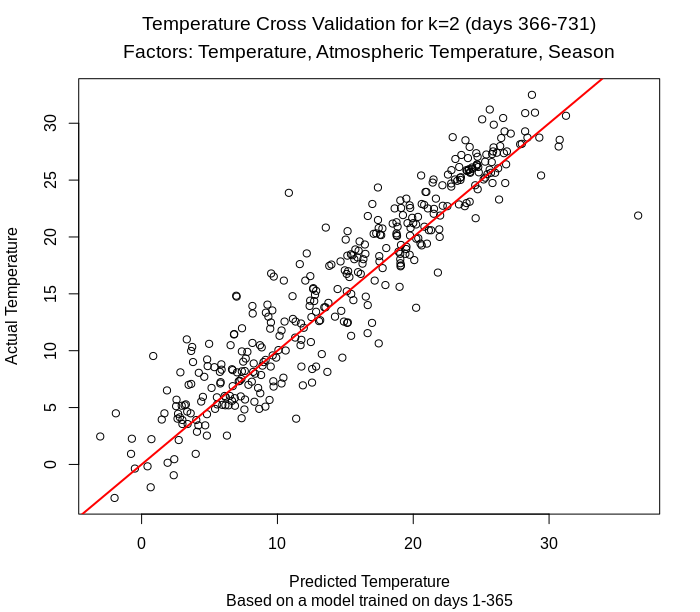
\includegraphics[width=.5\linewidth]{tempxvalidk=2.png} &   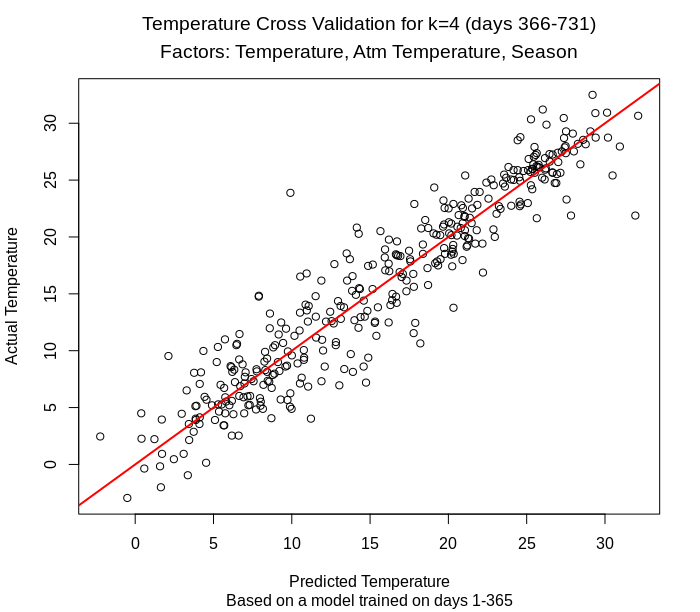
\includegraphics[width=.5\linewidth]{tempxvalidk=4.png} \\
(a) k = 3 & (b) k = 4 \\[6pt]
\end{tabular}
\caption{k = 2 vs k = 4}
\end{figure}

On the graph of k=4, we see that everything is slightly more compact and closer to the line. But most importantly, we see that there is a range of temperatures that are extremely close and densely located near the y=x line near ~26 degrees. However, the difference is still small. But, we can see a slight numerical improvement in R-squared value (k=2: 0.9203 vs k=4: 0.9271). 

However, when we compare k=4 to k=5 and k=4 to k=7, the differences are extremely minimal and hard to see.

\begin{figure}[H]
\begin{tabular}{cc}
  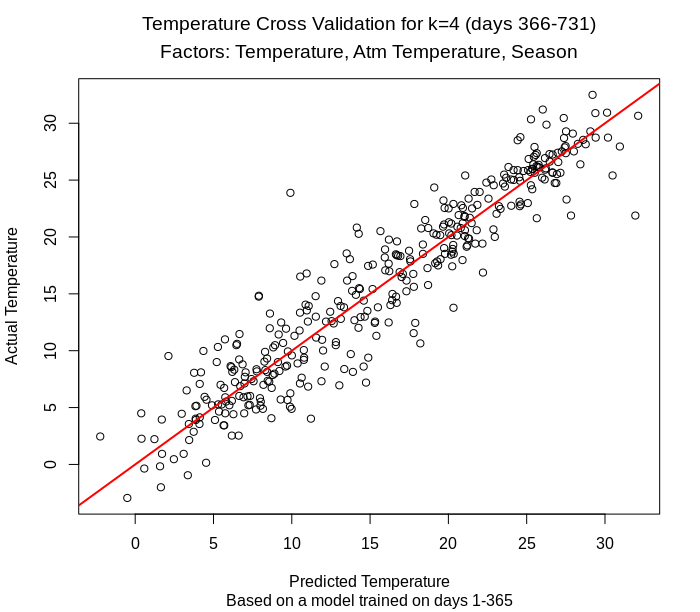
\includegraphics[width=.5\linewidth]{tempxvalidk=4.png} &   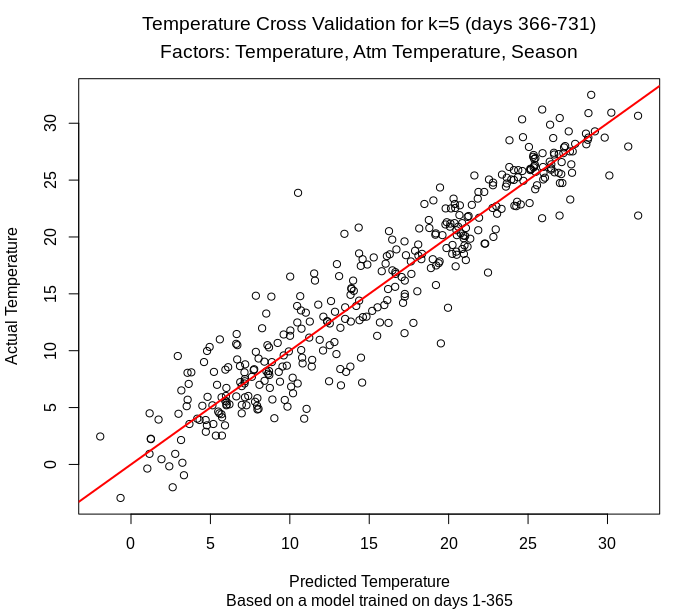
\includegraphics[width=.5\linewidth]{tempxvalidk=5.png} \\
(a) k = 4 & (b) k = 5 \\[6pt]
\end{tabular}
\caption{k = 4 vs k = 5}
\end{figure}

For example, taking a look between the graph of k=4 and k=5, we don't notice any drastic differences. Both data sets are relatively close to the y=x line, and they both share the same outlier. Therefore, we will compare the R-squared values to see which one is better on paper (of course R-squared isn't everything, and will be addressed later). k=4 has $0.9271$ while k=5 has $0.9294$. Therefore k=5 is "better" since it has a higher R-squared value, but in the end, it is negligible. Personally, I believe that having a lower k amongst two very similar models is more important, as it relies less on past data which reduces the risk of overfitting.

Finally, let's compare k=4 to k=7 to see who is the king.

\begin{figure}[H]
\begin{tabular}{cc}
  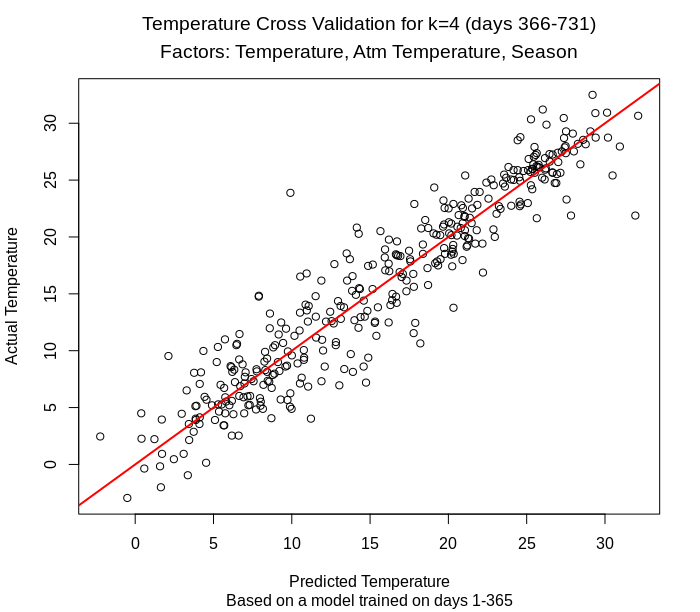
\includegraphics[width=.5\linewidth]{tempxvalidk=4.png} &   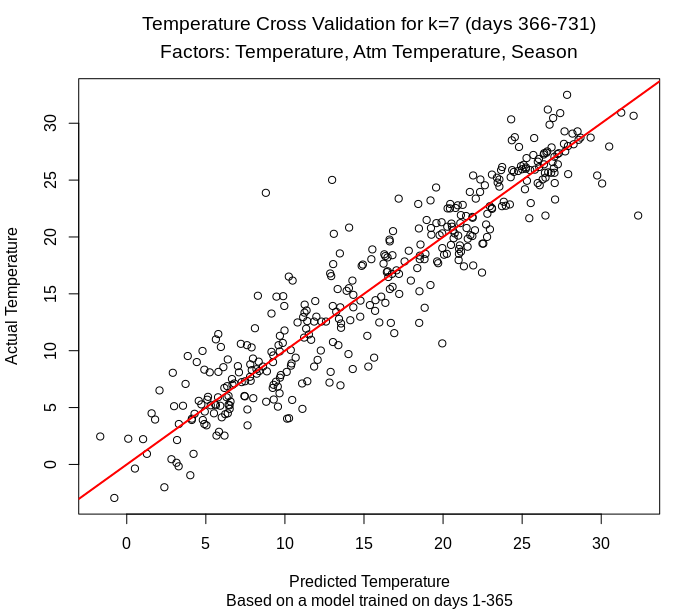
\includegraphics[width=.5\linewidth]{tempxvalidk=7.png} \\
(a) k = 4 & (b) k = 7 \\[6pt]
\end{tabular}
\caption{k = 4 vs k = 7}
\end{figure}

From this comparing k=7 against k=4, we can see that k=7 becomes a little bit more fuzzier. In other words, there are now extra points that are pushing the limits of becoming outliers. For example, near the middle, there are an extra couple of points that became further away from the line. This means that k=7 has slightly worse performance than k=4 which marks the decreasing of accuracy. However, we see something interesting, our R-squared values say the opposite. k=4 has $0.9271$ while k=7 has $0.9339$ which means that k=7 has a higher R-squared value!

Curious, I started testing the limits of how high R-squared could get until I arrived at k = 60 days. At k=60 days, we get an extremely beautiful R-squared value: $0.9994$ and the adjusted R-squared value is $0.9555$ which is still higher than all the previous k values.

\subsubsection{The Fallacy of R-squared Values}
Since k=60 has the highest R-squared value by far, even taking into account the adjusted R-squared value which tries to account for overfitting through too many predictor variables, I was excited since I found an extremely good value. That is until I cross-validated it.	

\begin{figure}[H]
	\centering
  	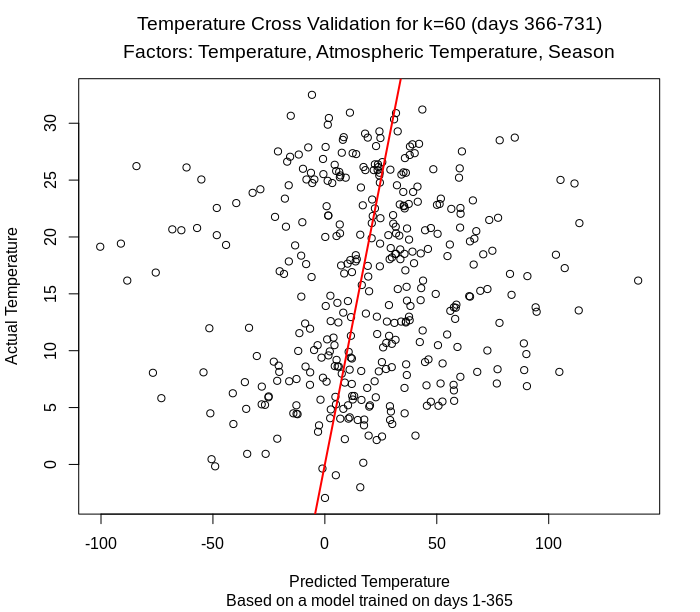
\includegraphics[width=150mm]{tempxvalidk=60.png}
 	\caption{Temperature Cross Validation for k = 60}
 	\label{fig:tempxvalidk=60}
\end{figure}

This graph shows the fallacy within R-squared values. Even though R-squared may be extremely high, it does not mean the model is good. In our case, the model failed in that there are many huge outliers that go to the -100 temperature range (we would become ice cubes). This is explained by how k=60 introduced 300 predictor variables which is a clear case of overfitting. But, R-squared is high because for our training set, the vast number of predictor variables are able to predict days within our training set accurately. This can be seen with this graph: 

\begin{figure}[H]
	\centering
  	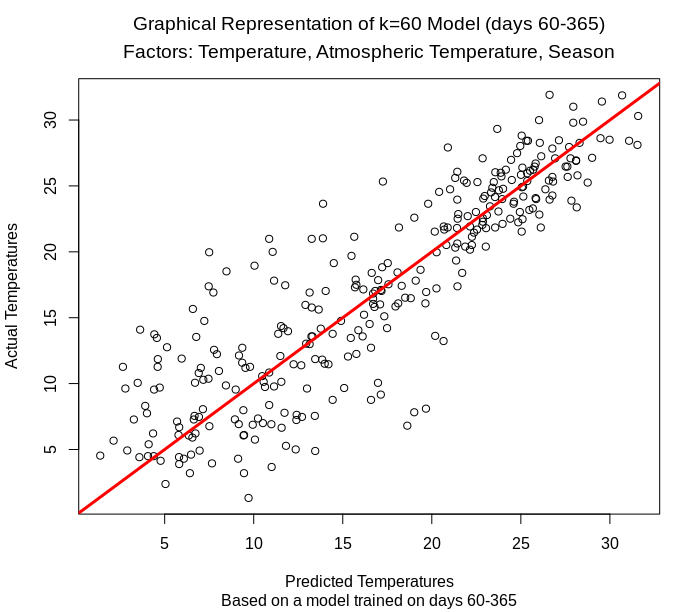
\includegraphics[width=150mm]{k=60model.png}
 	\caption{k = 60 for training data days}
 	\label{fig:k=60model}
\end{figure}

Oddly enough, even when we graph the graphical representation of the training set's predicted values, we get a bad result. A high R-squared value suggests that the points are extremely close to the line, but that seems to be the opposite.

In conclusion, k=60's R-squared value is a trap, and k=60 is the worst model we have discussed so far.

\subsubsection{Best Temperature Model: Th Final Verdict}
The best model found is k=4 and the predictive variables are Temperature, Atmospheric Temperature, and Seasons. This was chosen based on the R-squared value while making sure overfitting was not happening by cross-validating it. Additionally, it was chosen due to the relatively low amount of outliers it produced as well as the density of points around the y=x line.

\newpage
\subsection{Predicting Atmospheric Temperature (ATemp)} \label{predictingatemp}
\subsubsection{What Influences Atmospheric Temperature?} \label{atemp_params}
Now that we have discovered what influences temperature from Section \ref{temp_params}, it may seem like predicting atmospheric temperature would be similar since they both deal with temperature. However, this is not the case as there are some extra factors to consider when predicting atmospheric temperature.

First, it should be established that atmospheric temperature has a close relationship with temperature. This can be seen by overlaying atmospheric temperature vs days with temperature vs days.
\begin{figure}[H]
	\centering
  	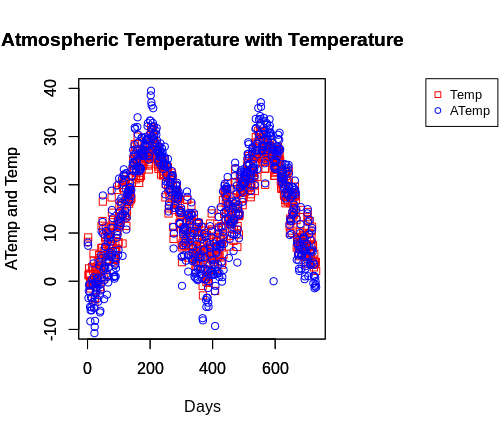
\includegraphics[width=150mm]{atempvstemp.png}
 	\caption{Atmospheric Temperature with Temperature Overlayed}
 	\label{fig:atempandtemp}
\end{figure}
As seen from this picture, we see that atmospheric temperature is highly reliant on temperature, but at the same time it also varies from temperature. This tells us that there are other factors that may contribute to atmospheric temperature's inflation or deflation.

Thinking about it scientifically, humidity would be one of the factors that contribute to atmospheric temperature's variation from temperature. This is caused by the fact that when it is very humid, to us humans, it feels very warm and hot. This will inflate the atmospheric temperature. However, on the other hand, when it is not humid at all, the air feels dry and cold to us.

Additionally, wind speed would be another one of the factors that contributes to the variation. When it is extremely windy to us, it feels a lot colder since there is a breeze.

However, to confirm that those factors are necessary, let's try graphing the model without taking into account humidity and wind speed.

\subsubsection{An "Alright" Model}
Since atmospheric temperature is very closely related to temperature (a correlation value of 0.99!), it is safe to assume that k=4 is the most optimal for it as well. However, we will test this further later on. But for this example, we will graph k=4 with the parameters Past Temperature, Past Atmospheric Temperature, and Season.

From doing the cross-validation technique described in Section \ref{finding}, we get the graph:

\begin{figure}[H]
	\centering
  	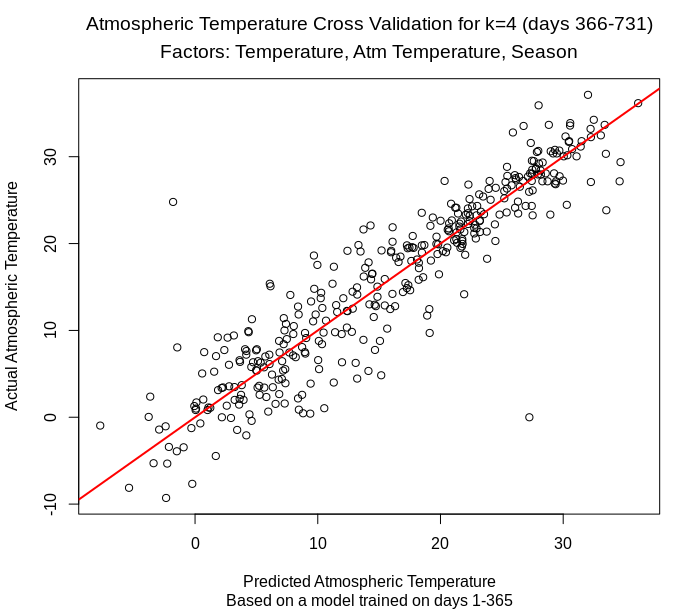
\includegraphics[width=130mm]{badatempxvalidk=4.png}
 	\caption{k = 4 without regard for humidity and wind speed}
 	\label{fig:badmodel}
\end{figure}

Looking at this graph, we note that there is somewhat a good relation between the predicted values and the actual values. However, the R-squared value is only $0.9157$ which could be improved.

\subsubsection{Improving Our "Alright" Model}
Firstly, as discussed in Section \ref{atemp_params}, we note that humidity and wind speed affect atmospheric temperature. So let's go ahead and create brand new models. While I'm at it, I will be trying to find the most optimal value of k again. However, I do suspect that k=4 is the most optimal since that was the most optimal value for temperature.

Following similar steps as Section \ref{finding}, we will go ahead and test multiple k values and analyze the graphs.

\begin{figure}[H]
\begin{tabular}{ccc}
  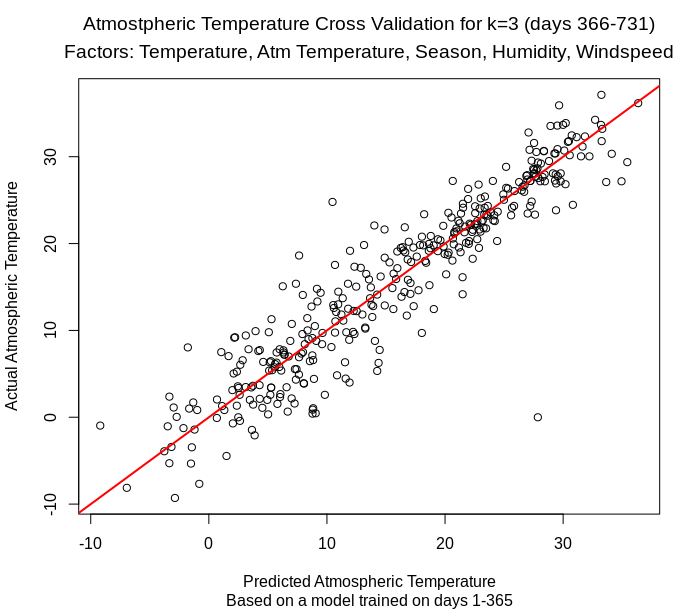
\includegraphics[width=.33\linewidth]{atempwindhumk=3.png} &  
  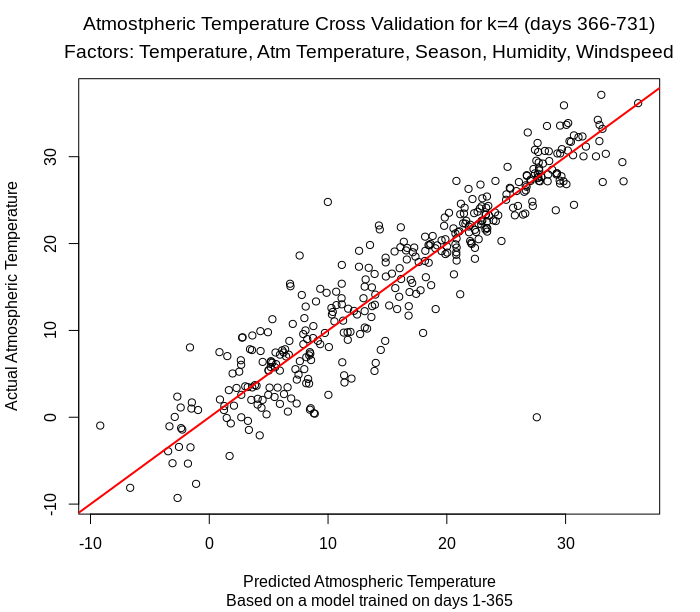
\includegraphics[width=.33\linewidth]{atempwindhumk=4.png} &   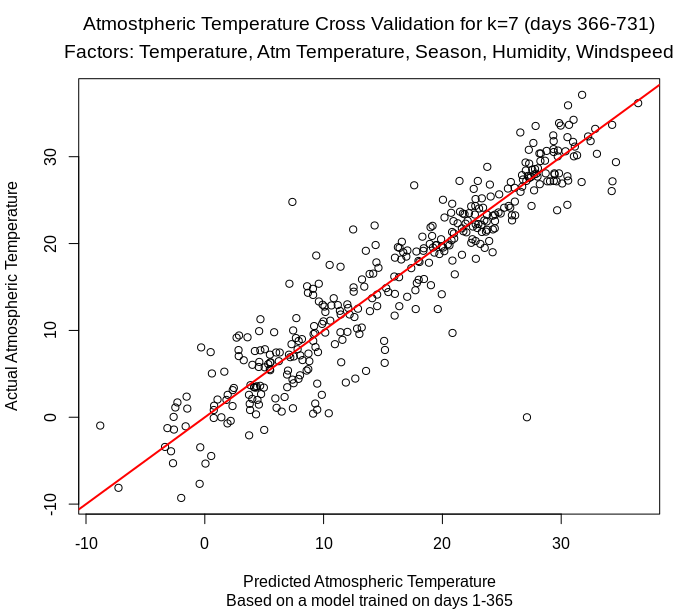
\includegraphics[width=.33\linewidth]{atempwindhumk=7.png} \\
(a) k = 3 & (b) k = 4 & (c) k = 7\\[6pt]
\end{tabular}
\caption{k = 3 vs k = 4 vs k = 7}
\label{atemphumresult}
\end{figure}

Once again, we see minimal difference from all three k values. However, this time, our k=3 model is a lot better than the temperature's k=3 model. We are able to see this if we compare them side by side.

\begin{figure}[H]
\begin{tabular}{cc}
  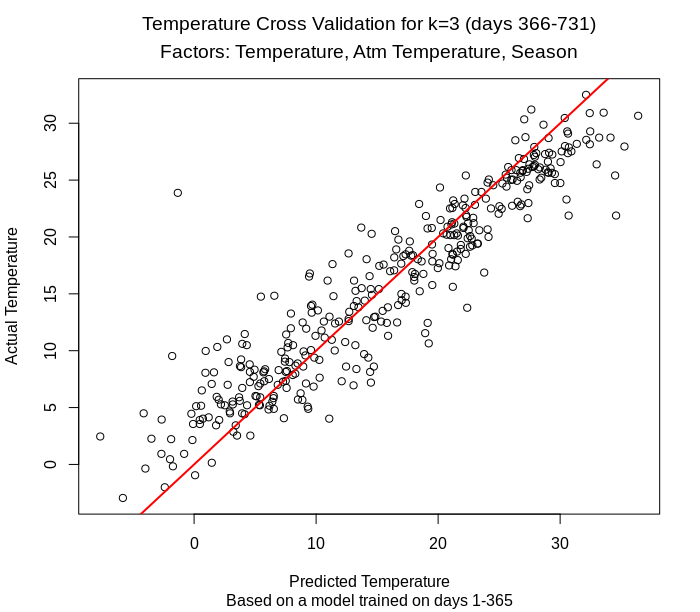
\includegraphics[width=.5\linewidth]{tempxvalidk=3.png} &  
  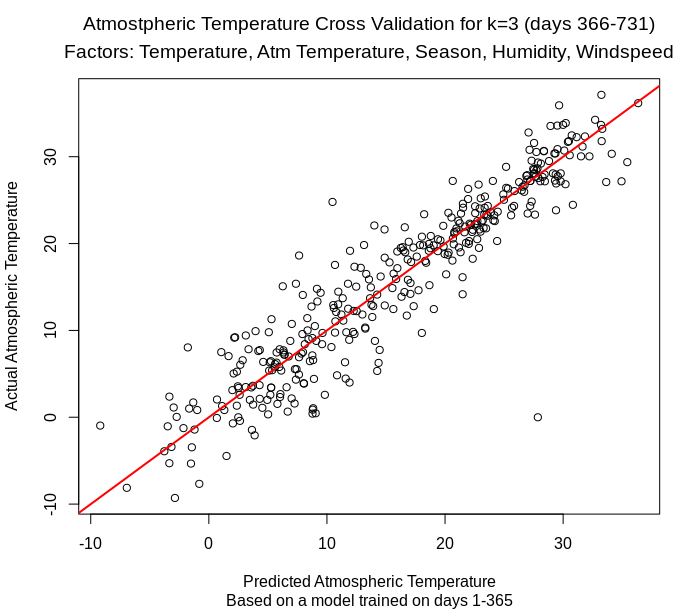
\includegraphics[width=.5\linewidth]{atempwindhumk=3.png} \\
(a) Temp's k = 3 & (b) ATemp's k = 3 \\[6pt]
\end{tabular}
\caption{Temp's k = 3 vs ATemp's k = 3}
\end{figure}

We can see temperature's k=3 graph falling in accuracy near the end, however atmospheric temperature's k=3 graph still predicts relatively accurately towards the end. Additionally, atmospheric temperature k=3 graph's points has more points that are closer to the line which gives it a more tight look.

Going back to analyzing which k value is the best, although there are very minimal differences, we can rely on R-squared since our k value is small enough for 3 and 4 so that it will not overfit. We note that k=3's R-squared value, $0.9226$, is slightly smaller than k=4's R-squared value, $0.9235$. This suggests that the k=4 model is bigger.

Comparing k=4 to k=7 brings up a similar situation to temperature's comparison of k=4 to k=7. k=7's R-squared value, $0.9299$, is larger than k=4's R-squared value, $0.9235$. However, this is a small increase compared the the number of predictor variables added when k=7 (21 variable increase) which could lead to overfitting. Additionally, k=7's adjusted R-squared value is only $0.001$ bigger which implies that adding that many more predictor variables will most likely not help the model that much. Therefore, k=4 is the most optimal value again.

However, there might be more ways we could improve the model.

\subsubsection{"Improving" Our Previous Improvement?}
Atmospheric temperature can also be influenced by weather conditions as well. For example, if it is super windy, or there is a thunder storm, then it would make atmospheric temperature plummet significantly. Therefore, let's try to create a model that takes into account weather conditions.

In day1, there are 4 weather condition categories, therefore we will make 3 dummy variables to represent each weather condition. A dummy variable for category 1, another for category 2, and a final one for category 3.

Using our optimal value of k=4, we will generate a model for atmospheric temperature with the parameters of the past temperatures, past atmospheric temperature, seasons, humidity, wind speed, and weather conditions.

However doing this, we run into a problem. Some of the coefficients are NA because of singularities. For example:
\begin{verbatim}
Coefficients: (4 not defined because of singularities)
                   Estimate Std. Error t value Pr(>|t|)    
(Intercept)         0.79014    3.50362   0.226   0.8217    
trainingdata[, 1]   0.08087    0.29580   0.273   0.7847    
trainingdata[, 2]   0.01988    0.22606   0.088   0.9300    
trainingdata[, 3]   1.68313    2.93331   0.574   0.5665    
trainingdata[, 4]   5.18911    3.34327   1.552   0.1216    
trainingdata[, 5]   2.90825    2.95880   0.983   0.3264    
trainingdata[, 6]   0.32224    1.73311   0.186   0.8526    
trainingdata[, 7]  -0.02837    0.04368  -0.649   0.5165    
trainingdata[, 8]  -0.94970    1.04587  -0.908   0.3645    
trainingdata[, 9]  -0.86795    0.94019  -0.923   0.3566    
trainingdata[, 10]       NA         NA      NA       NA    
trainingdata[, 11]  0.04882    0.33545   0.146   0.8844    
trainingdata[, 12]  0.03773    0.25087   0.150   0.8805    
trainingdata[, 13] -1.81253    4.18031  -0.434   0.6649    
trainingdata[, 14]  0.89647    4.66602   0.192   0.8478    
trainingdata[, 15]  0.71823    4.04004   0.178   0.8590    
trainingdata[, 16] -3.16594    1.93040  -1.640   0.1020    
trainingdata[, 17]  0.02363    0.04500   0.525   0.6000    
trainingdata[, 18]  0.04669    1.07571   0.043   0.9654    
trainingdata[, 19] -0.36723    0.95562  -0.384   0.7010    
trainingdata[, 20]       NA         NA      NA       NA    
...
\end{verbatim}

Inspecting this closely, we note that trainingdata[, 10] is actually the predictor variable for $weathersit == 3$, or in other words the weather condition being in category 3.

To understand why, we must look at how many times there are category 4 weathers.

\begin{verbatim}
> length(which(day1$weathersit[1:365] == 4))
[1] 0
\end{verbatim}

0 days in our training set have a weather category of 4. Therefore, in reality we actually have 3 categories total in our training set since the 4th category never occurs. Therefore, we need 2 dummy variables rather than 3.

Taking this change into account, we get:
\begin{figure}[H]
	\centering
  	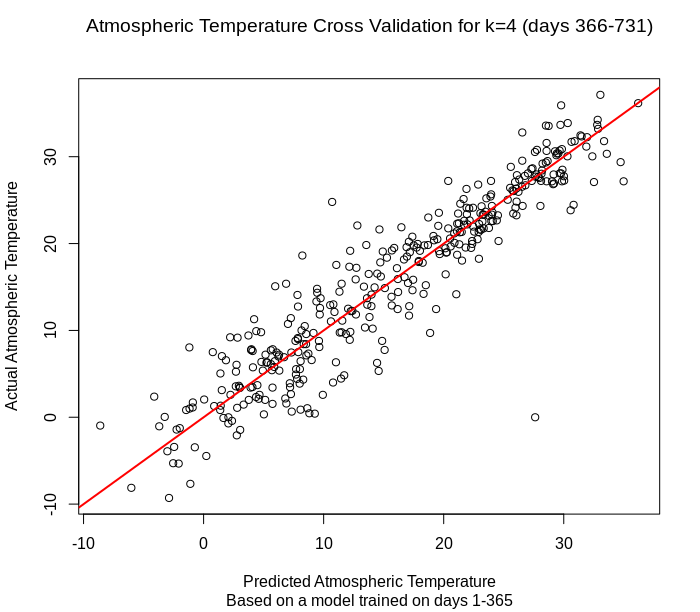
\includegraphics[width=150mm]{atempextrak=4.png}
 	\caption{k = 4 with the factors temperature, atmospheric temperature, seasons, humidity, wind speed, and weather conditions}
 	\label{fig:atempextra}
\end{figure}

Additionally we get a R-squared value of $0.9259$. Comparing this to our previous k=4 graph without the weather conditions, $0.9235$, it becomes apparent that perhaps including weather conditions is not as impactful as it seemed. Adding weather conditions to the model introduces and extra 8 predictor variables which is not worth the very slight increase by 0.002.

\subsubsection{Best Atmospheric Temperature Model: The Final Verdict}
By analyzing all of these possible predictor variables and values of k, it becomes clear that the most optimal and efficient model would be k=4 with the predictor variables Temperature, Atmospheric Temperature, Season, Humidity, and Wind Speed. This is due to the best-value R-squared value with respect to how many predictors are being used. It beat out k=3 with the same parameters, but still had a small enough number of predictor variables to not be overfit. This was confirmed by creating the cross-validation graph from Figure \ref{atemphumresult}(b).

\newpage
\subsection{Predicting Weathersit}
\subsubsection{Weathersit Overview}

The variable ``weathersit" is categorical, meaning that is discrete and has a 
number of defined states. Each of these states, of which there are four, describe the weather patterns on the day the data was taken. State 1 represents lightly cloudy or clear skies, 2 represents mist or overcast, 3 represents light rain or snow, and 4 represents heavy rain or snow. 

The categorical nature of our data poses a challenge because the typical usage of the K-Nearest Neighbors algorithm will not work. This is because the output will be continuous and not discrete like we want. Instead, we use dummy variables to create four different linear models, one for each of the four states. We normalize these to have a value between 0 and 1 and instead treat these values as the \textit{probability} that the day has the weather matching our model.

\subsubsection{Influencing Factors}
We are given 15 different variables that can influence weathersit, but which ones actually matter? With 15 variables, we have $15!$ or over 1 trillion different combinations of variables! It's effectively impossible to test them all, but we can start whittling down that number right away.

Clearly, the trial number has no indication of our weather, so we can remove the variable ``instant". Similarly, whether or not the day is a working day, a week day, or a holiday should not affect the weather, so we can remove the respective variables. 

Now our remaining variables are tricky. They all could be related to weathersit. Let's look at three variables in particular, humidity, windspeed, and the total number of bikes registered. The blue circles are our data points and the red line is the best fit line, which we will use to track their relationship.

\begin{figure}[H]
	\centering
  	\includegraphics[width=150mm]{"Weathersit Predicted by Humidity"}
 	\caption{Weathersit Predicted by Humidity}
 	\label{Weathersit Predicted by Humidity}
\end{figure}

In the case of humidity, there is a clear positive relationship with weathersit. Although it seems that there's
a lot of variance in our data, there is little relative to the other data sets we will be using. This means that humidity will likely be a strong predictor of weathersit.

\begin{figure}[H]
	\centering
  	\includegraphics[width=150mm]{"Weathersit Predicted by Windspeed"}
 	\caption{Weathersit Predicted by Windspeed}
 	\label{Weathersit Predicted by Windspeed}
\end{figure}

Unlike with humidity, windspeed seems to have little affect on weathersit. It has neither a positive nor negative relationship, meaning that it will likely be a poor indicator of weathersit. In addition, windspeed has much more variance than humidity, meaning that the relationship is more flimsy.

\begin{figure}[H]
	\centering
  	\includegraphics[width=150mm]{"Weathersit Predicted by Total Bikes Registered"}
 	\caption{Weathersit Predicted by Total Bikes Registered}
 	\label{Weathersit Predicted by Total Bikes Registered}
\end{figure}

Total bikes registered has a clear negative relationship with weathersit. This makes sense, as more people bike when its sunny than when its raining. Thus, it may seem that total bikes registered would be as good a predictor as humidity. However, there is a huge problem with its variance. It has an even higher variance than even windspeed, which means that the same value of total bikes registered could predict multiple states of weathersit.

From these graphs, we can predict that humidity will be a strong predictor, windspeed will be a poor predictor, and total bikes registered will be an average or good predictor. 

We can test this hypothesis by adding and removing these predictors to our model. Let's begin with a control model using only temp and atemp and see how our average accuracy changes when we add these variables. We evaluate each test with 100 trials and two models, a sequential model and a random model. The sequential model trains and tests on the data sequentially and with the data of previous day. The random model mixes up the data and test and trains on them in a random order.

\begin{table}[H]
\centering
 \begin{tabular}{||c | c c||} 
 \hline
 Variable Added & Sequential Model Accuracy & Random Model Accuracy \\ [0.5ex] 
 \hline\hline
 None (Control) & 0.56 & 0.60 \\ 
 Humidity & 0.72 & 0.70 \\
 Windspeed & 0.57 & 0.58 \\
 Total Bikes Registered & 0.64 & 0.63  \\ [1ex] 
 \hline
 \end{tabular}
\end{table}

As we guessed before, humidity is the best predictor, followed by total bikes registered and finally windspeed. Both humidity and total bikes registered increased the effectiveness of the model, whereas windspeed seemed to have a very marginal negative effect. The small affect of windspeed is most likely due to the reasons we stated earlier, especially the relatively small linear dependence. 

However, just because these factors are linearly related, that does not mean that they will be the best predictors in the final model. For that we need to find the best \textit{combination} of factors, all of which may influence each other. For this, we need to utilize another strategy.

\subsubsection{Comparing Models}
To create the best model, we need to utilize a lot of trial and error. We have evaluated each factor based on its linear relationship, which gave us a good place to start. However, we now need to find the best combination of factors.

We begin by combining all the effective linear variables together and seeing how those fare. These include, temp, atemp, humidity, and total bikes registered. Next, we can try using the effective linear variables and the bike variables, meaning the four variables above and the causual and registered bikes. Then we try the weather variables and the effective linear variables, meaning the four prior and windspeed. We also have one test using the time variables. We then compare all of them using a plot.

\begin{figure}[H]
	\centering
  	\includegraphics[width=150mm]{"Sequential Model Comparison"}
 	\caption{Sequential Model Comparison}
 	\label{Sequential Model Comparison}
\end{figure}

For the Sequential Model, we can clearly see that the weather data model, using temp, atemp, humidity, and windspeed is drastically more accurate than all other models. If we perform a little more trial and error, we find that we cannot improve this model by adding or removing any combination of two or less factors. It is possible that this is not the best model, but this is perhaps the closest we can get without testing all trillion combinations. 

\begin{figure}[H]
	\centering
  	\includegraphics[width=150mm]{"Random Model Comparison"}
 	\caption{Random Model Comparison}
 	\label{Random Model Comparison}
\end{figure}

For the Random Model, our results are a little different. The weather data model still performs well, but the linear model data, formed from temp, atemp, humidity, and total bikes registered, performs even better. This may be because our data is not a perfect sample. If we train sequentially, all the test data will be from a season/month/year combination that we have never seen before. 

With a random model, this is not a problem, as there is a high probability we will have trained on a few instances within that time period. With a sequential model, this becomes a big problem if the predicted time period is substantially different from the training set. With enough data (at least 2 or 3 years) we could likely avoid the problem with the sequential model and even be able to predict small changes in the next year, but its unlikely on this data set.

\subsubsection{The Best Model}
As stated before, the weather data is the best model in terms of combinations of factors. However, we still have more work to do. There are a number of \textit{hyper-parameters} which can be optimized to achieve an even better model. We have k, the number of nearest neighbors in our model, the size of our training data, and the number of previous days we use to predict the current day. 

It should be noted that the random model does not make perfect sense in this example. It is used more as a another method to test our models than as the desired output. This is because we're working with weather data, and thus, we want to be able to predict the current day's weather from the information of the past days. With the sequential model, up until this point, we have defaulted that value to three. This means we were using the predictor variables from the three previous days to predict the weather for the current day.

\begin{figure}[H]
	\centering
  	\includegraphics[width=150mm]{"Prediction Accuracy Distribution"}
 	\caption{Prediction Accuracy Distribution}
 	\label{Prediction Accuracy Distribution}
\end{figure}

With some more trial and error, we find that our optimized hyper-parameters are $k = 3$, $days \_ ago = 1$, and $num \_ training = 500$. This model gives us our greatest sequential model accuracy of $0.78$ and random model accuracy of $0.73$ averaged over 100 trials.

However, accuracy isn't always the best metric for fitness. What if we want to know how accurate the model is at predicting rain or clear skies? We can also show this by using the same method we used earlier for showing the relationships between various variables and weathersit. We can plot the linear relationship between our predicted weathersit and the actual weathersit.

\begin{figure}[H]
	\centering
  	\includegraphics[width=150mm]{"Seq Pred"}
 	\caption{Relationship Between Prediction and Actual}
 	\label{Relationship Between Prediction and Actual}
\end{figure}

This figure shows us the difference between the desired relationship (in orange) and our actual relationship (in blue). In addition, the correct predictions are pictured as circles in green and the incorrect predictions in red.

This plot shows us how accurate our model at predicting every type of weather. The further the blue line is from the orange line, the more inaccurate our predictions. If the blue line is above that represents over-prediction, and below represents under-prediction.

\subsubsection{Predicting Rain}
One thing which is clear right away from our weather data model is that it is quite good at predicting states 1 and 2, which is weather without rain or snow, and poor at predicting state 3, which is light snow and rain. 

There are a few reasons this might be. The first is our data set. As mentioned before, our sequential model does not get an even spread of the data, only a slice. So we may have a fewer percentage of rainy days than the average over the whole data set. However, if we look at the data, we find that to be false. Instead, we have a \textit{higher} percentage of rainy days in our training data.

\begin{table}[H]
\centering
 \begin{tabular}{||c | c c c c ||} 
 \hline
 Data Section & Winter & Spring & Summer & Fall \\ [0.5ex] 
 \hline\hline
 Total Rainy Days       & 4 & 3 & 4 & 10 \\ 
 Train Data Rainy Days  & 3 & 3 & 3 & 8 \\
 Test Data Rainy Days   & 1 & 0 & 1 & 2 \\
 Total Probability Rain & 0.55\% & 0.41\% & 0.55\% & 1.40\% \\
 Train Probability Rain & 0.60\% & 0.60\% & 0.60\% & 1.60\% \\
 Test Probability Rain  & 0.43\% & 0.00\% & 0.43\% & 0.087\% \\ [1ex] 
 \hline
 \end{tabular}
\end{table}

Based on this data, we would expect to over-predict the rainy days, as our training data has them in higher proportion. Instead, the opposite is true and we under-predict.

This could be because of the relatively few cases when the weather is actually rainy. Because there are so few, the KNN algorithm does not fit them into the model as much. Instead, we fit too much to the common states 1 and 2. This could be amended with an alternative model, but that model would likely lose out on overall accuracy. In addition, the random model could be effective at predicting rain, but we would lose the intention behind the model to predict the current day's weather from previous days.

\subsubsection{Conclusion}
The most effective KNN model we found for predicting weathersit utilized the predictors of temp, atemp, windspeed, and humidity.

\begin{table}[H]
\centering
 \begin{tabular}{||c | c c ||} 
 \hline
 Test Metric & Correct & False Positive \\ [0.5ex] 
 \hline\hline
 Overall   & 78.0\% & 22.0\% \\ 
 State 1   & 92.1\% & 24.5\% \\
 State 2   & 52.6\% & 18.4\% \\
 State 3   & 25.0\% & 0.00\% \\ [1ex] 
 \hline
 \end{tabular}
\end{table}

As shown above, this model predicted clear weather very accurately, but was poor at predicting rainy weather. 
In addition, the model was biased toward predicting clear weather, as shown by the fact that the percentage of false positives plus the percentage of correct predictions for state 1 was over 100\%. This means, we predicted state 1 more often than it showed up in the test data.

\newpage
\subsection{Predicting Humidity}
\subsubsection{The Pattern of Humidity}
Before creating a model to predict the humidity of a certain day, I checked if it had an obvious pattern over a week, month, or year. 

\begin{figure} [!h]
\centering
\begin{subfigure}{.5\textwidth}
  \centering
  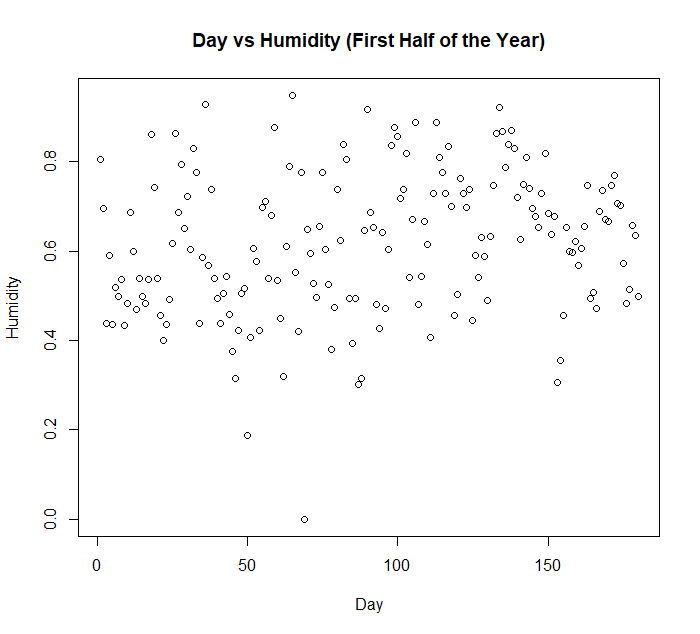
\includegraphics[width=1.05\linewidth]{DvsH1half.png}
  \caption{First Half of the Year}
  \label{fig:1half}
\end{subfigure}%
\begin{subfigure}{.5\textwidth}
  \centering
  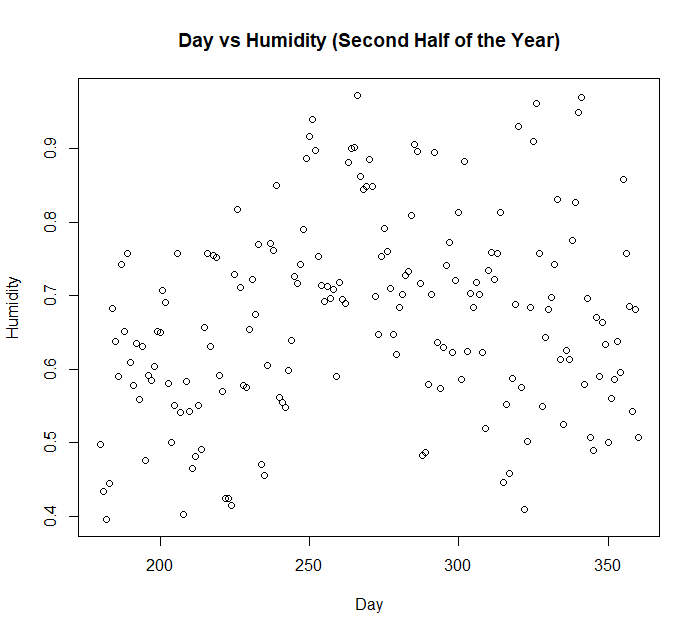
\includegraphics[width=1.05\linewidth]{DvsH2half.png}
  \caption{Second Half of the Year}
  \label{fig:2half}
\end{subfigure}
\caption{Day vs Humidity (One year)}
\label{fig:year}
\end{figure}


Upon inspecting the graph of humidity over the course of a year, there is no obvious pattern that can be deduced about humidity in the first half of the year, whereas there is a more distinct pattern in the second half of the year. In Figure \ref{fig:1half}, the data seems to be very sporadic and random. On the other hand, the overall shape of Figure \ref{fig:2half} subtly resembles a wide, upside-down U. However, this pattern could be highly coincidental. This means that a definitive statement cannot be made about the pattern of humidity in the second half of any year. Because of this, we have to look at humidity over the course of a smaller time span; we decided to check if there was a pattern over consecutive months.

\begin{figure}[H]
\centering
\begin{subfigure}{.5\textwidth}
  \centering
  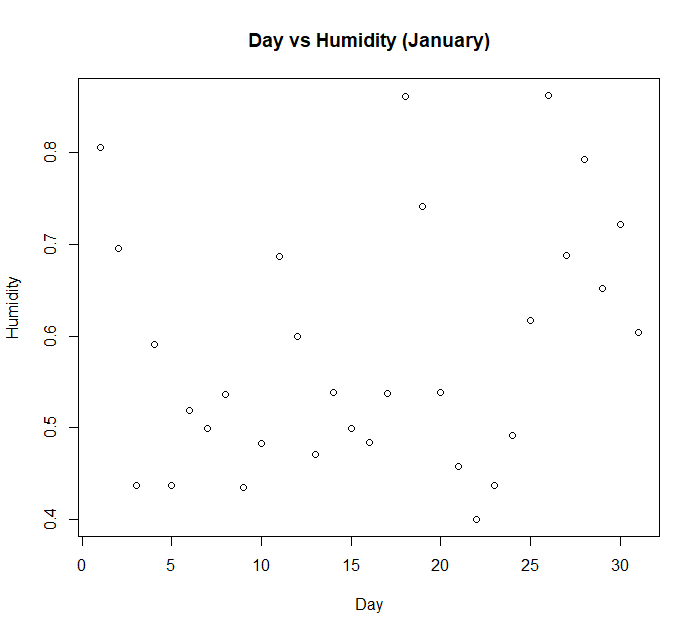
\includegraphics[width=1.05\linewidth]{DvsHjan.png}
  \caption{January}
  \label{fig:jan}
\end{subfigure}%
\begin{subfigure}{.5\textwidth}
  \centering
  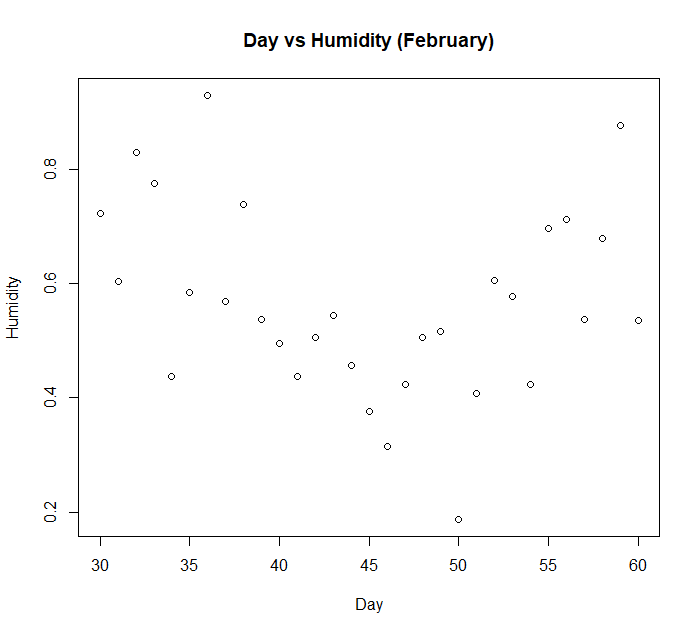
\includegraphics[width=1.05\linewidth]{DvsHfeb.png}
  \caption{February}
  \label{fig:feb}
\end{subfigure}
\caption{Day vs Humidity (January vs February)}
\label{fig:2mon}
\end{figure}

In Figure \ref{fig:2mon}, the humidity resembles a wave-like pattern. However, because these graphs do not share a common shape, no conclusion can be made about the behavior of humidity over a month. In addition, the data could also be highly coincidental, and no fact can be made about how humidity behaves in every January or February. This means that humidity has to be inspected even further. This caused us to look at how humidity behaves over a few days, or a week. 

\begin{verbatim}
> day1$hum[1:7]

  0.805833 0.696087 0.437273 0.590435 0.436957 0.518261 0.498696

> day1$hum[33:39]

  0.775417 0.437826 0.585217 0.929167 0.568333 0.738333 0.537917
\end{verbatim}


In the first week of January, the humidity peaks on the first day at 0.805833, decreases for the next two days, and then increases on the fourth day. For the next three days, the humidity has a decrease-increase-decrease pattern. This pattern can also be seen in one of the weeks of February. From this data, it is clear that humidity makes random jumps, at seemingly unpredictable intervals, at random times. Because the amount of increase and decrease between each day is not consistent, and appears to be random, humidity will be difficult to predict.  

\subsubsection{Factors That Affect Humidity}
Despite the sporadic nature of humidity, there are some factors that can affect it. Among the given variables in the data set, the main variables that can affect humidity are temperature, atmospheric temperature, and the current season.  

The reason for temperature being chosen is that there is a general relationship between temperature and humidity. Usually, when the temperature increases, the amount of water vapor in the air increases, which means that the humidity also increases. In addition, when the temperature decreases, the humidity also decreases. 

Likewise, atmospheric temperature also has a relationship with humidity. When the atmospheric temperature is high, the humidity will also be high. To add, when the atmospheric temperature is low, the humidity will also be low.

Lastly, since both temperature and atmospheric temperature are related to the current season (lower temperatures during winter, and higher temperatures during summer), the current season plays a role in affecting humidity. We will use dummy variables for each season.

\subsubsection{Creating the model}

Using the first year of the data set as my training set, we used the lm() function to create a model used to predict the humidity of each day in the second year. Due to the sporadic  nature of humidity, and its inconsistent jumps between each day, we figured that the most recent data, the past 2 days, will help provide the best prediction. Thus, we decided to use the last 2 days (k = 2) to predict the current humidity.

In order to visualize the difference between using temperature and atmospheric temperature to predict humidity, separate graphs were created with each of them being the sole driving force of the training set. In addition, to see how accurate the model is, the predicted humidity was compared against the actual humidity.

\begin{figure} [H]
\centering
\begin{subfigure}{.5\textwidth}
  \centering
  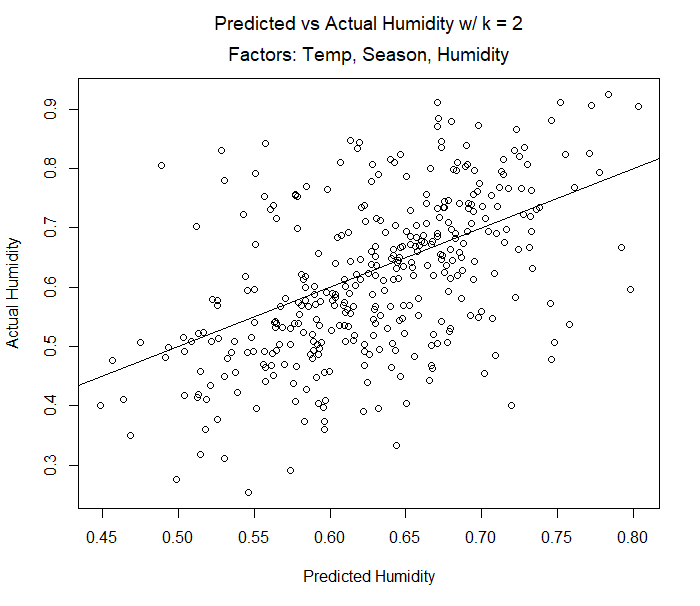
\includegraphics[width=70mm]{TvsH.png}
  \caption{Using Temperature}
  \label{fig:tvh}
\end{subfigure}%
\begin{subfigure}{.5\textwidth}
  \centering
  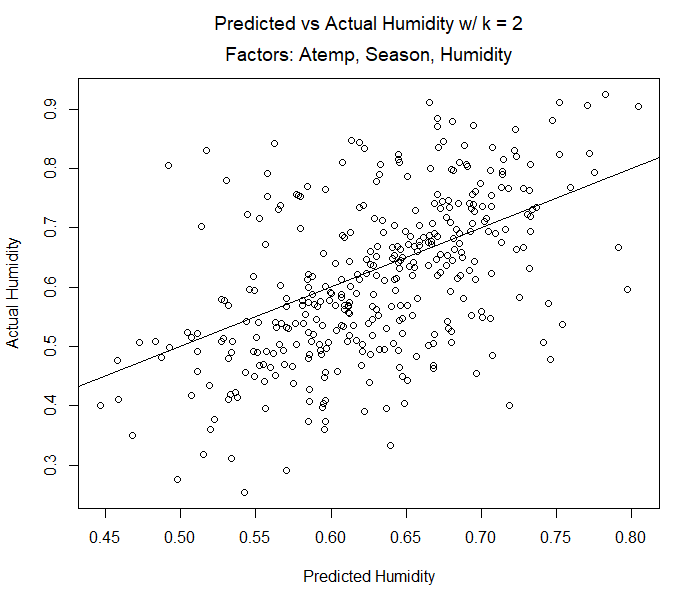
\includegraphics[width=70mm]{ATvsH.png}
  \caption{Using Atmospheric Temperature}
  \label{fig:atvh}
\end{subfigure}
\caption{Predicted vs Actual Humidity}
\label{fig:tempvsh}
\end{figure}

As seen in Figure \ref{fig:tempvsh}, both graphs are nearly identical. Moreover, the same sporadic nature of humidity is apparent since there are many data points spread throughout the whole graph, including many outliers. Thus, this model is not the best at predicting humidity, and it must be improved by changing the predictor variables.

\subsubsection{Improving the model}

Upon thinking about temperature and atmospheric temperature, we suspected that what people would feel outside is the difference between the two. In turn, this is also related to humidity, as we normally feel warmer when the humidity is higher. This lead us to use the difference between temperature and atmospheric as our predictor variable, in replacement of just the temperature or atmospheric temperature.

\begin{figure} [H]
	\centering
  	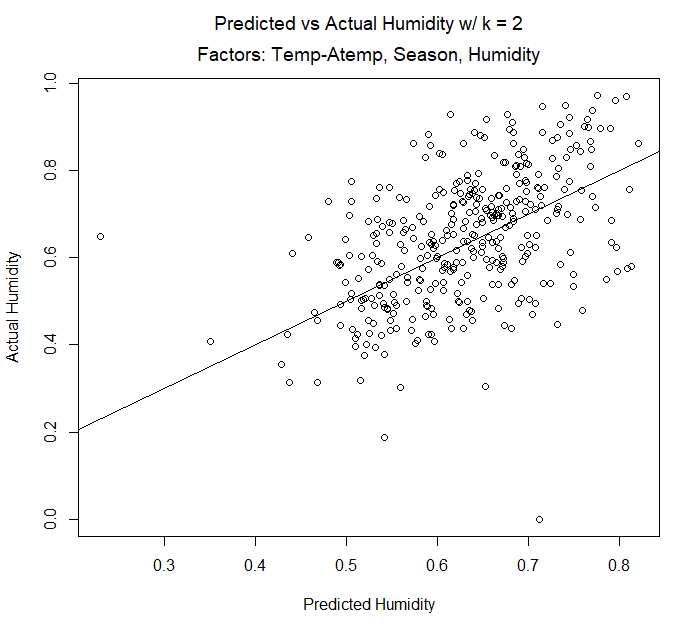
\includegraphics[width=100mm]{T-ATvsH.png}
 	\caption{Predicted Humidity vs Actual Humidity}
 	\label{fig:t-at}
\end{figure}

Compared to Figure \ref{fig:tempvsh}, the data points are more centralized around an area. However, the data is still very spread out, and contains many outliers. As seen in this graph, there is still some randomness between the humidity of each consecutive day. Although this model is an improvement to the previous model by a slight margin, it is still not the best model for predicting humidity. Despite this, we know that humidity is not completely random as it is affected by temperature and atmospheric temperature. In order to see how each predictor variable affects our humidity prediction, we need to look at the magnitude of how each predictor variable affects our response variable. To dig  even further, let's look at the coefficients of this model.

\begin{verbatim}
> summary(lmout)

Call:
lm(formula = currhum ~ temp2ago + temp1ago + hum2ago + (hum1ago) + 
    winter + spring + summer)

Residuals:
     Min       1Q   Median       3Q      Max 
-0.66153 -0.07382  0.00966  0.08023  0.33248 

Coefficients:
             Estimate Std. Error t value Pr(>|t|)    
(Intercept)  0.436587   0.044312   9.853  < 2e-16 ***
temp2ago     0.005387   0.006563   0.821  0.41230    
temp1ago    -0.018132   0.006487  -2.795  0.00547 ** 
hum2ago     -0.053058   0.052686  -1.007  0.31459    
hum1ago      0.442161   0.053205   8.310 2.05e-15 ***
winter      -0.051043   0.022178  -2.302  0.02194 *  
spring      -0.013724   0.019250  -0.713  0.47636    
summer      -0.013424   0.020252  -0.663  0.50784    
---
Signif. codes:  0 ‘***’ 0.001 ‘**’ 0.01 ‘*’ 0.05 ‘.’ 0.1 ‘ ’ 1

Residual standard error: 0.1274 on 355 degrees of freedom
Multiple R-squared:  0.282,	Adjusted R-squared:  0.2678 
F-statistic: 19.91 on 7 and 355 DF,  p-value: < 2.2e-16
\end{verbatim}

To note, "temp2ago" and "temp1ago" actually represent abs(temp-atemp) for each day.
After glancing at the values of the coefficients, it is apparent that the coefficient of "hum1ago", the humidity from the previous day, has the greatest value. With a coefficient of 0.442161, which is about eight times as much as the absolute value of the next greatest coefficient, the humidity from one day ago plays the most important role in predicting the current humidity. Among the seasons, winter has the smallest coefficient, -0.051043. This makes sense since both the temperature and atmospheric temperature are usually the lowest during the winter, and that the humidity would drop even more during this season. 
In addition, this model has a R-squared value of 0.282, which is relatively low. Considering how spread out the data points are, this value makes sense. This means that this model is far from being an adequate one for predicting humidity. Furthermore, the inconsistent jumps between each days' humidity has also contributed to this low R squared value.  

Next, we decided to test if increasing the recentness of the data would improve our prediction of the humidity. Here, we have a graph using the five most recent days (k = 5).

\begin{figure} [!h]
	\centering
  	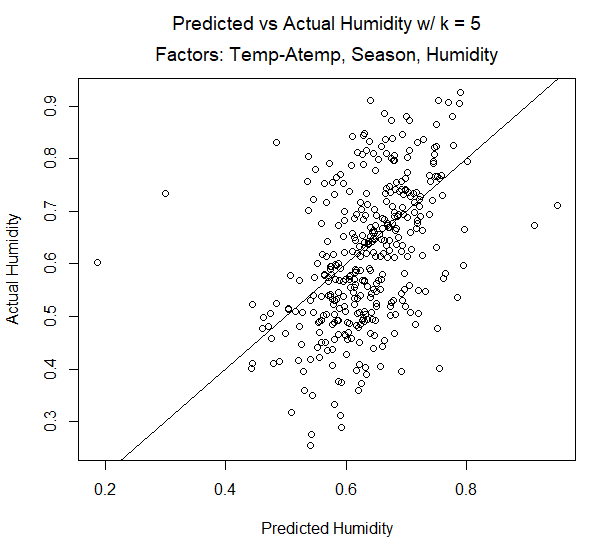
\includegraphics[width=75mm]{T-ATk5.png}
 	\caption{Predicted Humidity vs Actual Humidity; k = 5}
 	\label{fig:t-atk5}
\end{figure} 	

Compared to Figure \ref{fig:t-at}, using a recentness of 5 days does not improve our model. In this graph, the points are more spread out and contains more outliers. Since, increasing the recentness of the data does not improve the prediction of humidity, it is better to use a smaller value of k.
 
\subsubsection{Concluding Thoughts}
As seen from the graphs in beginning, the humidity of a certain day can have a large increase or decrease from its previous day. Thus, humidity must be looked at on a day-to-day basis. Simply looking at it over the course of a year or a month is not helpful as humidity doesn't have a distinct pattern over a long time span. Although humidity can jump sporadically, it is not completely random since humidity is affected by both the temperature and atmospheric temperature. In terms of recentness, it is better to use data from one or two days ago. This means that any more data past these two days will probably result in a more inaccurate prediction of humidity, since the current humidity may or may not differ by a large amount from the previous day's humidity. To add, using the absolute value of the difference between the temperature and atmospheric temperature as our predicted variable has improved the model, than using them separately. 
 
\newpage
\subsection{Predicting Wind Speed}
\subsubsection{Factors Affecting Wind Speed}

Among the variables in the data set, the main factors that affect wind speed is temperature, atmospheric temperature, and the current season.

How does temperature affect wind speed?
Since the main component that affects wind speed is air pressure, which is affected by temperature differences, temperature has a role in affecting wind speed. The larger the temperature difference, the larger the air pressure, and thus the stronger the winds will be.  

How does atmospheric temperature affect wind speed?
Atmospheric temperature has an inverse relationship with wind speed. As the atmospheric temperature decreases, the effects of the wind increases. This means that at lower atmospheric temperatures, the winds would feel stronger and have a higher wind speed.

How does the current season affect temperature?
As previously stated, the temperature and season are strongly related (greater temperatures during the summer, and lower temperatures during the winter). Thus, the 
season plays a role in affecting wind speed.

\subsubsection{Creating the model}

The predictor variables for our model consists of temperature, atmospheric temperature, wind speed, and the season. For the season, we will use dummy variables for winter, spring, and summer. The training set will consist of data from the first year of the data set. In terms of recentness, we used the started with the two most recent days (k = 2). First, we used the lm() function in R to generate a basic model used to predict wind speed, then compared the predicted wind speeds to the actual wind speeds.

\subsubsection{Comparing the effects of Temperature and Atmospheric Temperature}
Starting off, in order to visualize which predictor variable, temperature or atmospheric temperature, would be better for our prediction model, we created a graph for each one.

\begin{figure} [H]
	\centering
  	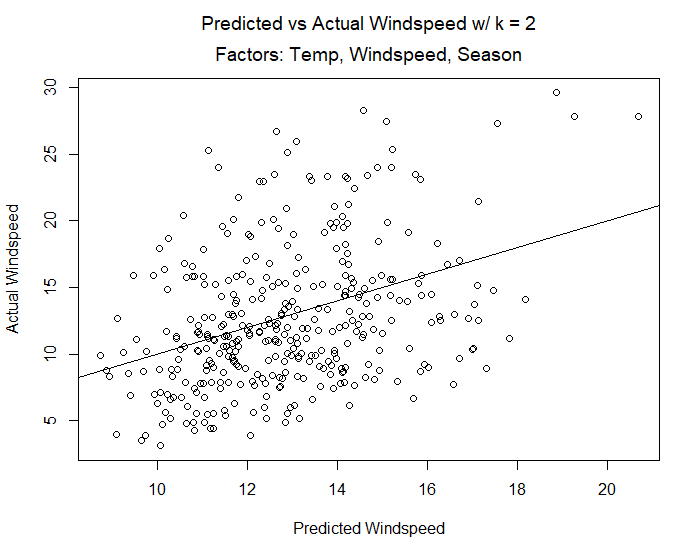
\includegraphics[width=74mm]{TempWs.png}
 	\caption{Using Temperature}
 	\label{fig:tvws}
\end{figure} 

\begin{figure} [!h]
	\centering
  	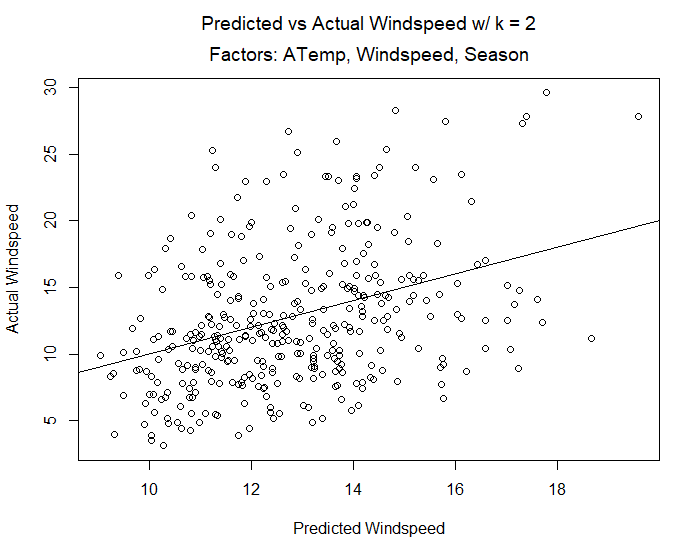
\includegraphics[width=74mm]{AtempWs.png}
 	\caption{Using Atmospheric Temperature}
 	\label{fig:atvws}
\end{figure} 


From Figures \ref{fig:tvws} and \ref{fig:atvws}, we can see that both graphs look nearly identical. In both of the graphs, the data is very spread out and contains many outliers. However, in the Figure \ref{fig:atvws}, there are more points around abline(0,1), and the data points are very slightly more closer to the center. Despite this, the differences between each graph could be regarded as negligible since there is no significant change that we can notice. Nonetheless, both graphs in Figures \ref{fig:tvsws} and \ref{fig:atvws} do not convey a model that accurately predicts wind speed.

\subsubsection{Improving the model}

To improve our model, we decided to use the absolute value of the difference between temperature and atmospheric temperature as our predictor variable.   
 
\begin{figure} [!h]
	\centering
  	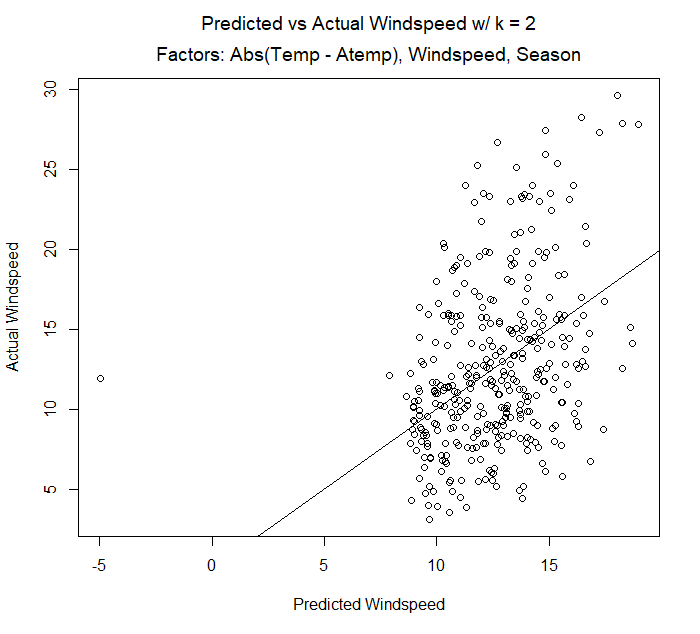
\includegraphics[width=90mm]{T-Awk2.png}
 	\caption{Abs(Temp - Atemp)}
 	\label{fig:tawk2}
\end{figure} 

With the exception of the extreme outlier near the far left edge, the data points in Figure \ref{fig:tawk2} are more centralized than the ones in Figures \ref{fig:tvws} and \ref{fig:atvws}. 

\begin{verbatim}
> summary(lmout)

Call:
lm(formula = currws ~ atemp2ago + atemp1ago + +ws2ago + (ws1ago) + 
    winter + spring + summer)

Residuals:
     Min       1Q   Median       3Q      Max 
-12.0487  -3.4890  -0.5067   3.0052  17.8593 

Coefficients:
            Estimate Std. Error t value Pr(>|t|)    
(Intercept)  8.17170    1.09144   7.487 5.62e-13 ***
atemp2ago   -0.09315    0.08044  -1.158  0.24763    
atemp1ago    0.11887    0.08140   1.460  0.14510    
ws2ago      -0.03103    0.05506  -0.564  0.57338    
ws1ago       0.27921    0.05296   5.272 2.35e-07 ***
winter       2.52157    0.81105   3.109  0.00203 ** 
spring       1.72909    0.79189   2.183  0.02965 *  
summer       0.06188    1.00126   0.062  0.95075    
\end{verbatim}

To note, "atemp2ago" and "atemp1ago" actually represent abs(temp-atemp) for each day.
Based on these coefficients, it seems that the wind speeds are greatest during the winter. This makes sense since temperatures during the winter are lower, which causes the atmospheric temperature to decrease, and thus increase the wind speed. In addition, the coefficients for "ws1ago" and "atemp1ago" are also greater than "ws2ago" and "atemp2ago". This insinuates that the previous days data play a more significant in predicting the wind speed for the next day. This pattern was also seen in the prediction model regarding humidity. When it comes to recentness, it seems that the most recent day, the previous day, provides the most accurate data for prediction.


\subsubsection{Adjusting Recentness}
Can our model be improved by adjusting the recentness to include more days?

Here, we will compare the graphs between using the 3 most recent days and the 5 most recent days.

\begin{figure} [H]
\centering
\begin{subfigure}{.5\textwidth}
  \centering
  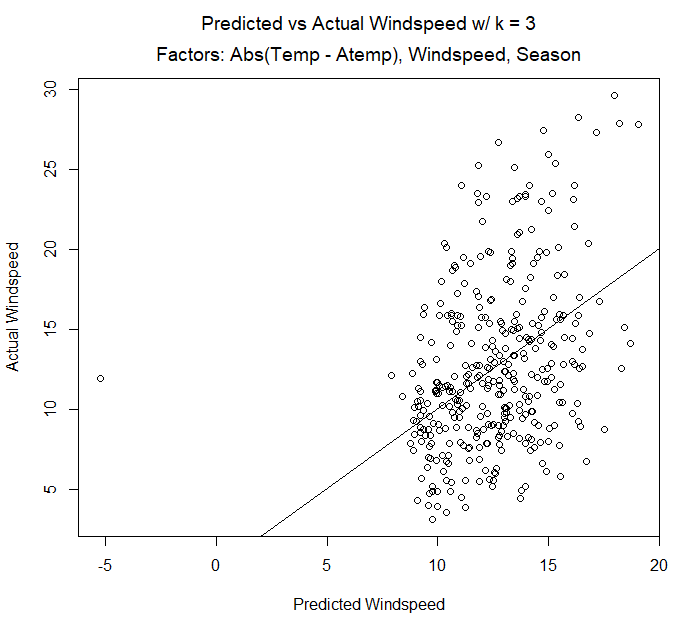
\includegraphics[width=80mm]{T-Awk3.png}
  \caption{k = 3}
  \label{fig:wsk3}
\end{subfigure}%
\begin{subfigure}{.5\textwidth}
  \centering
  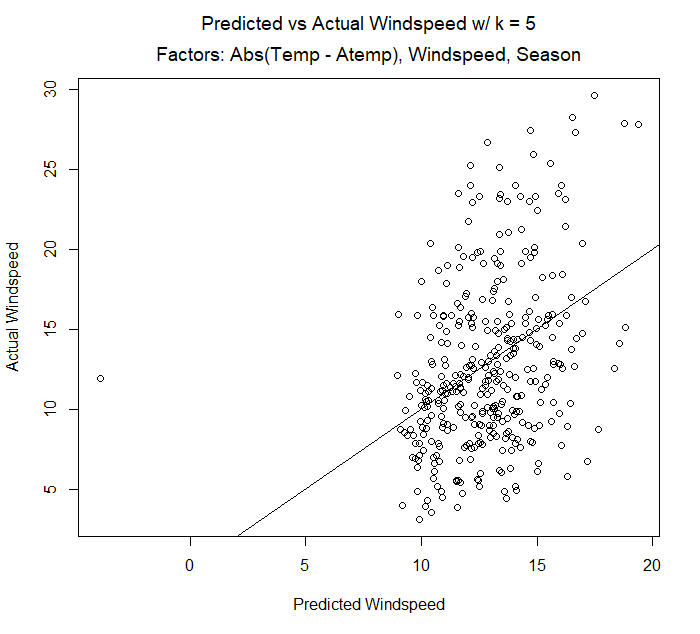
\includegraphics[width=80mm]{T-Awk5.png}
  \caption{k = 5}
  \label{fig:wsk5}
\end{subfigure}
\caption{Adjusting recentness}
\label{fig:3vs5}
\end{figure}

When comparing Figure \ref{fig:3vs5} to Figure \ref{fig:tawk2}, the graph changes very slightly when more days are used in the training set. On the first glance, the difference between them is negligible.

\begin{verbatim}
> summary(lmoutk3)
...
Multiple R-squared:  0.1508,	Adjusted R-squared:  0.1291 
...

> summary(lmoutk5)
...
Multiple R-squared:  0.1536,	Adjusted R-squared:  0.1218 
...
\end{verbatim}
Considering that both R-squared values, 0.1508 and 0.1536, are nearly the same, it is safe to say that increasing the amount of recent days we use in our training set does not result in a more accurate model

\subsubsection{Concluding Thoughts}

Using the absolute value of the difference between the temperature and atmospheric temperature as a predictor variable has resulted in a better model. In addition, keeping the amount of recent days to 2 allows for a more accurate prediction than increasing it. Furthermore, it seems that the season plays a big role in predicting wind speed, since both temperature and atmospheric temperature vary during different seasons. This could explain why the coefficients for the seasons in the model were the greatest. In the end, this model is still not perfect, as it can still be improved. For possible improvements, including the weather situation as a predictor variable would perhaps result in better predictions. For example, thunderstorms, heavy rains, and snowy situations can also affect wind speeds. 

\newpage
\section{Group Members and Their Roles}
\subsection*{Vincent Boc}
\begin{itemize}
\item Created the Latex Document and its structure.
\item The prelude to predicting temperature, sections \ref{disclaimer}, \ref{goal}, \ref{criteria}.
\item The entirety of predicting temperature (\ref{predictingtemp}) and atmospheric temperature (\ref{predictingatemp})
\item The following code files: tempModel.R, atempModel.R. season.R
\end{itemize}

\subsection*{Derek Li}
\begin{itemize}
\item Part B: Humidity
\item Part B: Wind speed
\end{itemize}

\subsection*{Nikhil Razdan}
\begin{itemize}
\item Analysis of parent dominion and offspring quality poster in section 1.2
\item Created model to predict weathersit in weathersit.R
\item Analysis of created weathersit model in section 2.6
\end{itemize}

\newpage
\appendix 
\section{tempModel.R}
\begin{lstlisting}[language=R]
runLMTemp <- function(trainingdataset) {
  k <- (ncol(trainingdataset) - 1) / 5
  xnam <- paste0("trainingdata[,", 1:(k * 5), "]")
  res <- lm(as.formula(paste0("trainingdata[,", k * 5 + 1,"] ~",
  		 paste0(xnam, collapse="+"))))
  return(res)
}

createTrainingDataTemp <- function(k) {
  trainingdata <- matrix(ncol=(k * 5 + 1), nrow=(365 - k))
  for (i in (k+1):365) {
    colTracker <- k * 5
    for (j in 1:k) {
      trainingdata[i - k, colTracker - 4] <- day1$temp[i - j]
      trainingdata[i - k, colTracker - 3] <- day1$atemp[i - j]
      trainingdata[i - k, colTracker - 2] <- as.integer(day1$season[i - j] 		
      	== 1)
      trainingdata[i - k, colTracker - 1] <- as.integer(day1$season[i - j] 
      	== 2)
      trainingdata[i - k, colTracker] <- as.integer(day1$season[i - j] == 3)
      colTracker <- colTracker - 5
    }
    trainingdata[i - k, k * 5 + 1] <- day1$temp[i]
  }
  print(trainingdata)
  return(trainingdata)
}

crossValidateTemp <- function(coefficients, k) {
  print(length(coefficients))
  values <- rep(0, 731 - 365)
  print(length(values))
  for (i in 1:(731 - 365)) {
    values[i] <- predictTemp(i + 365, coefficients, k)
    print(values[i])
  }
  return(values)
}

predictTemp <- function(day, coefficients, k) {
  winter <- as.integer(day1$season == 1)
  spring <- as.integer(day1$season == 2)
  summer <- as.integer(day1$season == 3)
  curr <- coefficients[1]
  i <- day
  daytracker <- 0
  for (j in seq(2, length(coefficients), 5)) {
    diff <- coefficients[j] * day1$temp[i - k + daytracker] +
    		coefficients[j+1] * day1$atemp[i - k + daytracker] +
    		coefficients[j+2] * winter[i - k + daytracker] + 
    		coefficients[j+3] * spring[i - k + daytracker] + 
    		coefficients[j+4] * summer[i - k + daytracker]
    curr <- curr + diff
    daytracker <- daytracker + 1
  }
  print(paste0("Final Prediction: ", curr, " Actual Temp: ", day1$temp[i]))
  return(curr)
}
\end{lstlisting}

\section{atempModel.R} 
\begin{lstlisting}[language=R]
runLMATemp <- function(trainingdataset, k) { # load trainingdata into trainingdata var
  xnam <- paste0("trainingdata[,", 1:(k * 7), "]")
  res <- lm(as.formula(paste0("trainingdata[,", k * 7 + 1,"] ~", 	
  	paste0(xnam, collapse="+"))))
  return(res)
}

createTrainingDataATemp <- function(k) {
  trainingdata <- matrix(ncol=(k * 7 + 1), nrow=(365 - k))
  print(dim(trainingdata))
  for (i in (k+1):365) {
    colTracker <- k * 7
    for (j in 1:k) {
      trainingdata[i - k, colTracker - 6] <- day1$temp[i - j]
      trainingdata[i - k, colTracker - 5] <- day1$atemp[i - j]
      trainingdata[i - k, colTracker - 4] <- as.integer(day1$season[i - j] 
      	== 1)
      trainingdata[i - k, colTracker - 3] <- as.integer(day1$season[i - j] 
      	== 2)
      trainingdata[i - k, colTracker - 2] <- as.integer(day1$season[i - j] 
      	== 3)
      trainingdata[i - k, colTracker - 1] <- day1$hum[i - j]
      trainingdata[i - k, colTracker] <- day1$windspeed[i - j]
      colTracker <- colTracker - 7
    }
    trainingdata[i - k, k * 7 + 1] <- day1$atemp[i]
  }
  return(trainingdata)
}

runModifiedLMATemp <- function(trainingdataset, k) { # load trainingdata into trainingdata var first
  xnam <- paste0("trainingdata[,", 1:(k * 9), "]")
  res <- lm(as.formula(paste0("trainingdata[,", k * 9 + 1,"] ~", paste0(xnam, collapse="+"))))
  return(res)
}

modifiedCreateTrainingDataATemp <- function(k) {
  trainingdata <- matrix(ncol=(k * 9 + 1), nrow=(365 - k))
  print(dim(trainingdata))
  for (i in (k+1):365) {
    colTracker <- k * 9
    for (j in 1:k) {
      trainingdata[i - k, colTracker - 8] <- day1$temp[i - j]
      trainingdata[i - k, colTracker - 7] <- day1$atemp[i - j]
      trainingdata[i - k, colTracker - 6] <- 
      	as.integer(day1$season[i - j] == 1)
      trainingdata[i - k, colTracker - 5] <- 
      	as.integer(day1$season[i - j] == 2)
      trainingdata[i - k, colTracker - 4] <- 
      	as.integer(day1$season[i - j] == 3)
      trainingdata[i - k, colTracker - 3] <- day1$hum[i - j]
      trainingdata[i - k, colTracker - 2] <- day1$windspeed[i - j]
      trainingdata[i - k, colTracker - 1] <- 
      	as.integer(day1$weathersit[i - j] == 1)
      trainingdata[i - k, colTracker] <- 
      	as.integer(day1$weathersit[i - j] == 2)
      colTracker <- colTracker - 9
    }
    trainingdata[i - k, k * 9 + 1] <- day1$atemp[i]
  }
  return(trainingdata)
}

crossValidateModifiedATemp <- function(coefficients, k) {
  print(length(coefficients))
  values <- rep(0, 731 - 365)
  print(length(values))
  for (i in 1:(731 - 365)) {
    values[i] <- predictModifiedATemp(i + 365, coefficients, k)
    print(values[i])
  }
  return(values)
}


predictModifiedATemp <- function(day, coefficients, k) {
  winter <- as.integer(day1$season == 1)
  spring <- as.integer(day1$season == 2)
  summer <- as.integer(day1$season == 3)
  clear <- as.integer(day1$weathersit == 1)
  cloudy <- as.integer(day1$weathersit == 2)
  curr <- coefficients[1]
  i <- day
  daytracker <- 0
  for (j in seq(2, length(coefficients), 9)) {
    diff <- coefficients[j] * day1$temp[i - k + daytracker] + 
    		coefficients[j+1] * day1$atemp[i - k + daytracker] + 
    		coefficients[j+2] * winter[i - k + daytracker] + 
    		coefficients[j+3] * spring[i - k + daytracker] + 
    		coefficients[j + 4] * summer[i - k + daytracker] +
    		coefficients[j + 5] * day1$hum[i - k + daytracker] +
    		coefficients[j + 6] * day1$windspeed[i - k + daytracker] + 
    		coefficients[j + 7] * clear[i - k + daytracker] + 
    		coefficients[j + 8] * cloudy[i - k + daytracker]
    curr <- curr + diff
    daytracker <- daytracker + 1
    
  }
  print(paste0("Final Prediction: ", curr, " Actual Temp: ", 
  	day1$atemp[i]))
  return(curr)
}


crossValidateATemp <- function(coefficients, k) {
  print(length(coefficients))
  values <- rep(0, 731 - 365)
  print(length(values))
  for (i in 1:(731 - 365)) {
    values[i] <- predictATemp(i + 365, coefficients, k)
    print(values[i])
  }
  return(values)
}

predictATemp <- function(day, coefficients, k) {
  winter <- as.integer(day1$season == 1)
  spring <- as.integer(day1$season == 2)
  summer <- as.integer(day1$season == 3)
  curr <- coefficients[1]
  i <- day
  daytracker <- 0
  for (j in seq(2, length(coefficients), 7)) {
    diff <- coefficients[j] * day1$temp[i - k + daytracker] + 	
    		coefficients[j+1] * day1$atemp[i - k + daytracker] + 	
    		coefficients[j+2] * winter[i - k + daytracker] + 
    		coefficients[j+3] * spring[i - k + daytracker] + 
    		coefficients[j + 4] * summer[i - k + daytracker] +
      		coefficients[j + 5] * day1$hum[i - k + daytracker] + 
      		coefficients[j + 6] * day1$windspeed[i - k + daytracker]
    curr <- curr + diff
    daytracker <- daytracker + 1
  }
  print(paste0("Final Prediction: ", curr, " Actual Temp: ", 
  	day1$atemp[i]))
  return(curr)
}

runBadLMATemp <- function(trainingdata, k) {
  xnam <- paste0("trainingdata[,", 1:(k * 5), "]")
  res <- lm(as.formula(paste0("trainingdata[,", k * 5 + 1,"] ~", 
  	paste0(xnam, collapse="+"))))
  return(res)
}

badCreateTrainingDataATemp <- function(k) {
  trainingdata <- matrix(ncol=(k * 5 + 1), nrow=(365 - k))
  
  for (i in (k+1):365) {
    colTracker <- k * 5
    for (j in 1:k) {
      trainingdata[i - k, colTracker - 4] <- day1$temp[i - j]
      trainingdata[i - k, colTracker - 3] <- day1$atemp[i - j]
      trainingdata[i - k, colTracker - 2] <- 
      	as.integer(day1$season[i - j] == 1)
      trainingdata[i - k, colTracker - 1] <- 
      	as.integer(day1$season[i - j] == 2)
      trainingdata[i - k, colTracker] <- 
      	as.integer(day1$season[i - j] == 3)
      colTracker <- colTracker - 5
    }
    trainingdata[i - k, k * 5 + 1] <- day1$atemp[i]
  }
  return(trainingdata)
} 


badCrossValidateTemp <- function(coefficients, k) {
  print(length(coefficients))
  values <- rep(0, 731 - 365)
  print(length(values))
  for (i in 1:(731 - 365)) {
    values[i] <- badPredictTemp(i + 365, coefficients, k)
    print(values[i])
  }
  return(values)
}

badPredictTemp <- function(day, coefficients, k) {
  winter <- as.integer(day1$season == 1)
  spring <- as.integer(day1$season == 2)
  summer <- as.integer(day1$season == 3)
  curr <- coefficients[1]
  i <- day
  daytracker <- 0
  for (j in seq(2, length(coefficients), 5)) {
    diff <- coefficients[j] * day1$temp[i - k + daytracker] + 
    		coefficients[j+1] * day1$atemp[i - k + daytracker] + 
    		coefficients[j+2] * winter[i - k + daytracker] + 
    		coefficients[j+3] * spring[i - k + daytracker] + 
    		coefficients[j + 4] * summer[i - k + daytracker]
    curr <- curr + diff
    daytracker <- daytracker + 1
  }
  print(paste0("Final Prediction: ", curr, " Actual Temp: ", 	
  		day1$atemp[i]))
  return(curr)
}
\end{lstlisting}

\section{season.R}
\begin{lstlisting}[language=R]
seasonanalysis <- function() {
  res <- rep(0, 8)
  names(res) <- c("Winter Mean", "Winter Median",
                     "Spring Mean", "Spring Median",
                     "Summer Mean", "Summer Median",
                     "Fall Mean", "Fall Median")
  res[1] <- mean(day1$temp[which(day1$season == 1)])
  res[2] <- median(day1$temp[which(day1$season == 1)])
  
  res[3] <- mean(day1$temp[which(day1$season == 2)])
  res[4] <- median(day1$temp[which(day1$season == 2)])
  
  res[5] <- mean(day1$temp[which(day1$season == 3)])
  res[6] <- median(day1$temp[which(day1$season == 3)])
  
  res[7] <- mean(day1$temp[which(day1$season == 4)])
  res[8] <- median(day1$temp[which(day1$season == 4)])
  return(res)
}
\end{lstlisting}

\section{humidity.R}
\begin{lstlisting} [language=R]
runHumidity <- function(){
library(regtools)
data(day1)
day1 <- day1[,c(3,9,10,11,12,13)]
head(day1)

temp3ago <- abs(day1$temp[1:362]-day1$atemp[1:362])
temp2ago <- abs(day1$temp[2:363]-day1$atemp[2:363])
temp1ago <- abs(day1$temp[3:364]-day1$atemp[3:364])
hum3ago <- day1$hum[1:362]
hum2ago <- day1$hum[2:363]
hum1ago <- day1$hum[3:364]
currhum <- day1$hum[4:365]
winter <- as.integer(day1$season[4:365] == 1)
spring <- as.integer(day1$season[4:365] == 2)
summer <- as.integer(day1$season[4:365] == 3)
seasons <- cbind(winter, spring, summer)
inside3x <- cbind(temp3ago, temp2ago, temp1ago, 
                  hum3ago, hum2ago, hum1ago,
                  seasons)
lmout <- lm(currhum ~ temp3ago+temp2ago+temp1ago+
              hum3ago+hum2ago+(hum1ago)
            +winter+spring+summer)

otemp3ago <- abs(day1$temp[366:728]-day1$atemp[366:728])
otemp2ago <- abs(day1$temp[367:729]-day1$atemp[367:729])
otemp1ago <- abs(day1$temp[368:730]-day1$atemp[368:730])
ohum3ago <- day1$hum[366:728]
ohum2ago <- day1$hum[367:729]
ohum1ago <- day1$hum[368:730]
ocurrhum <- day1$hum[369:731]
owinter <- as.integer(day1$season[369:731] == 1)
ospring <- as.integer(day1$season[369:731] == 2)
osummer <- as.integer(day1$season[369:731] == 3)
oseasons <- cbind(owinter, ospring, osummer)
outside2x <- cbind(otemp3ago,otemp2ago,otemp1ago, 
                   ohum3ago,ohum2ago, ohum1ago, oseasons)

predictxx <- rep(0,363)
startday <- 1
for (rep in 1:363) {
  predictxx[rep] <- predictxx[rep] + lmout$coefficients[1]
  for (co in 2:9) {
    predictxx[rep] <- predictxx[rep] + lmout$coefficients[co] * outside2x[startday,co-1]
  }
  startday <- startday + 1
}

plot(predictxx, day1$hum[369:731], xlab = "Predicted Humidity", ylab = "Actual Humidity", main = bquote(atop("Predicted vs Actual Humidity w/ k = 3", "Factors: Abs(Temp-Atemp), Season, Humidity")))
abline(0,1)
}
\end{lstlisting}

\section{windspeed.R}
\begin{lstlisting} [language=R]
runWindSpeed <- function(){
library(regtools) 
data(day1)

day1 <- day1[,c(1,2,3,9,10,11,12,13)]
head(day1)

temp2ago <- abs(day1$temp[1:363] - day1$atemp[1:363])
temp1ago <- abs(day1$temp[2:364] - day1$atemp[2:364])
ws2ago <- day1$windspeed[1:363]
ws1ago <- day1$windspeed[2:364]
currws <- day1$windspeed[3:365]
winter <- as.integer(day1$season[3:365] == 1)
spring <- as.integer(day1$season[3:365] == 2)
summer <- as.integer(day1$season[3:365] == 3)
inside <- cbind(temp2ago, temp1ago, atemp2ago, atemp1ago, ws2ago, ws1ago)
lmout <- lm(currws ~ atemp2ago+atemp1ago+
                      +ws2ago+(ws1ago)+
                      winter+spring+summer)

oatemp2ago <- abs(day1$atemp[367:729])
oatemp1ago <- abs(day1$atemp[368:730])
ows2ago <- day1$windspeed[367:729]
ows1ago <- day1$windspeed[368:730]
ocurrws <- day1$windspeed[369:731]
winter <- as.integer(day1$season[369:731] == 1)
spring <- as.integer(day1$season[369:731] == 2)
summer <- as.integer(day1$season[369:731] == 3)
o2x <- cbind(oatemp2ago, oatemp1ago, 
             ows2ago, ows1ago,
             winter,spring,summer)

predictxx <- rep(0,363)
startday <- 1
for (rep in 1:363) {
  predictxx[rep] <- predictxx[rep] + lmout$coefficients[1]
  for (co in 2:7) {
    predictxx[rep] <- predictxx[rep] + lmout$coefficients[co] * o2x[startday,co-1]
  }
  startday <- startday + 1
}

plot(predictxx, day1$windspeed[369:731], xlab = "Predicted Windspeed", ylab = "Actual Windspeed", 
     main = bquote(atop("Predicted vs Actual Windspeed w/ k = 2", "Factors: Abs(Temp-ATemp), Windspeed, Season")))
abline(0,1)
}


\end{lstlisting}

\section{weathersit.R} 
\begin{lstlisting}[language=R]
# Plotting simple linear relationships
plot_linear_relationships <- function() {
  plot(day1$weathersit, day1$hum, col = "blue", main = "Weathersit Predicted by Humidity",
       xlab = "Weathersit", ylab = "Humidity")
  abline(lm(day1$hum ~ day1$weathersit), col = "red")
  
  plot(day1$weathersit, day1$windspeed, col = "blue", main = "Weathersit Predicted by Windspeed",
       xlab = "Weathersit", ylab = "Windspeed")
  abline(lm(day1$windspeed ~ day1$weathersit), col = "red")
  
  plot(day1$weathersit, day1$tot, col = "blue", main = "Weathersit Predicted by Total Bikes Registered",
       xlab = "Weathersit", ylab = "Total Bikes Registered")
  abline(lm(day1$tot ~ day1$weathersit), col = "red")
}

### SEQUENTIAL
sim_sequential <- function(num_training, predictors, k, days_ago, plot = NULL) {
  
  # getting test and train x
  trainx <- day1[1:num_training,predictors]
  testx <- day1[(num_training + 1):nrow(day1),predictors]
  
  # adding days_ago data
  for(i in 1:days_ago) {
      data <- day1[1:nrow(day1),predictors]
      for(j in 1:i) {
        data <- rbind(rep(NA, length(predictors)), data)
      }
      trainx <- cbind(trainx, data[1:num_training, ])
      testx <- cbind(testx, data[num_training:(nrow(data) - (i + 1)), ])
  }
  
  # creating test and train y data
  trainy <- day1$weathersit[1:num_training]
  testy <- day1$weathersit[(num_training + 1):nrow(day1)]
  
  # training and evaluating models
  knn_1 <- basicKNN(trainx,as.integer(trainy == 1),testx,k)
  knn_2 <- basicKNN(trainx,as.integer(trainy == 2),testx,k)
  knn_3 <- basicKNN(trainx,as.integer(trainy == 3),testx,k)
  knn_4 <- basicKNN(trainx,as.integer(trainy == 4),testx,k)
  knn_all <- data.frame(knn_1$regests, knn_2$regests, knn_3$regests, 
  knn_4$regests)
  colnames(knn_all) <- c(1, 2, 3, 4)
    
  # getting model predictions
  predictions <- colnames(knn_all)[max.col(knn_all,ties.method="first")]
  predictions <- strtoi(predictions)
  
  # Plot accuracy for all predictions
  if(!is.null(plot)) {
    plot(testy, predictions, 
         main = "Prediction vs Actual - Sequentially Chosen Data", 
         xlab = "Actual Weathersit", ylab = "Predicted Weathersit",
         xlim = c(1, 3), ylim = c(1,3), 
         col = ifelse(testy == predictions, "green", "red"))
    
    abline(lm(testy ~ predictions), col = "blue")
    lines(c(1, 2, 3), c(1, 2, 3), col = "orange")
  }

  # calculate and return accuracy
  accuracy <- sum(testy == predictions) / length(testy)
  return(accuracy)
}

### RANDOM
sim_random <- function(num_training, predictors, k, plot = NULL) {
  
  # getting random values
  rand <- sample(nrow(day1), nrow(day1), replace = FALSE)
  
  # getting test and train x data
  trainx <- day1[rand[1:num_training],predictors]
  testx <- day1[rand[(num_training + 1):nrow(day1)],predictors]
  
  # creating test and train y data
  trainy <- day1$weathersit[rand[1:num_training]]
  testy <- day1$weathersit[rand[(num_training + 1):nrow(day1)]]
  
  # training and evaluating models
  knn_1 <- basicKNN(trainx,as.integer(trainy == 1),testx,k)
  knn_2 <- basicKNN(trainx,as.integer(trainy == 2),testx,k)
  knn_3 <- basicKNN(trainx,as.integer(trainy == 3),testx,k)
  knn_4 <- basicKNN(trainx,as.integer(trainy == 4),testx,k)
  knn_all <- data.frame(knn_1$regests, knn_2$regests, knn_3$regests, 
                        knn_4$regests)
  colnames(knn_all) <- c(1, 2, 3, 4)
  
  # getting model predictions
  predictions <- colnames(knn_all)[max.col(knn_all,ties.method="first")]
  predictions <- strtoi(predictions)
  
  # Plot accuracy for all predictions
  if(!is.null(plot)) {
    plot(testy, predictions, main = "Prediction vs Actual - Randomly Chosen Data", 
         xlab = "Actual Weathersit", ylab = "Predicted Weathersit",
         xlim = c(1, 3), ylim = c(1,3), 
         col = ifelse(testy == predictions, "green", "red"))
    
    abline(lm(testy ~ predictions), col = "blue")
    lines(c(1, 2, 3), c(1, 2, 3), col = "orange")
  }
  
  # calculate and return accuracy
  accuracy <- sum(testy == predictions) / length(testy)
  return(accuracy)
}

seq_model_comparison <- function(num_training, nreps, k, days_ago) {
  linear_data <- rep(0.00, nreps)
  bike_data <- rep(0.00, nreps)
  weather_data <- rep(0.00, nreps)
  time_data <- rep(0.00, nreps)
  
  linear_predictors <- c(10, 11, 12, 16)
  bike_predictors <-  c(10, 11, 14, 15, 16)
  weather_predictors <- c(10, 11, 12, 13)
  time_predictors <- c(10, 11, 3, 4, 5)
  
  for(i in 1:nreps) {
    linear_data[i] <- sim_sequential(num_training, linear_predictors, k, days_ago)
    bike_data[i] <- sim_sequential(num_training, bike_predictors, k, days_ago)
    weather_data[i] <- sim_sequential(num_training, weather_predictors, k, days_ago)
    time_data[i] <- sim_sequential(num_training, time_predictors, k, days_ago)
  }
  
  boxplot(linear_data, bike_data, weather_data, time_data, 
          col = c("blue", "red", "green", "orange"), 
          main = "Prediction Accuracy Distribution", 
          names = c("Linear Data", "Bike Data", "Weather Data", "Time Data"), 
          xlab = "Data Type", 
          ylab = "Prediction Accuracy")
}

rand_model_comparison <- function(num_training, nreps, k, days_ago) {
  linear_data <- rep(0.00, nreps)
  bike_data <- rep(0.00, nreps)
  weather_data <- rep(0.00, nreps)
  time_data <- rep(0.00, nreps)
  
  linear_predictors <- c(10, 11, 12, 16)
  bike_predictors <-  c(10, 11, 14, 15, 16)
  weather_predictors <- c(10, 11, 12, 13)
  time_predictors <- c(10, 11, 3, 4, 5)
  
  for(i in 1:nreps) {
    linear_data[i] <- sim_random(num_training, linear_predictors, k)
    bike_data[i] <- sim_random(num_training, bike_predictors, k)
    weather_data[i] <- sim_random(num_training, weather_predictors, k)
    time_data[i] <- sim_random(num_training, time_predictors, k)
  }
  
  boxplot(linear_data, bike_data, weather_data, time_data, 
          col = c("blue", "red", "green", "orange"), 
          main = "Prediction Accuracy Distribution", 
          names = c("Linear Data", "Bike Data", "Weather Data", "Time Data"), 
          xlab = "Data Type", 
          ylab = "Prediction Accuracy")
}

main <- function() {
  print(sim_sequential(num_training, predictors, k, days_ago))
  print(sim_random(num_training, predictors, k))
  
  seq_data <- rep(0.00, nreps)
  rand_data <- rep(0.00, nreps)
  
  # Run nreps models and find average for sequential and random models
  for(i in 1:nreps) {
    seq_data[i] <- sim_sequential(num_training, predictors, k, days_ago)
    rand_data[i] <- sim_random(num_training, predictors, k)
    cat("Completed model", i, "\n")
  }
  
  plot(1:nreps, seq_data, col = "red", main = "Prediction Accuracy Over 100 Trials", 
       xlab = "Trial Number", ylab = "Prediction Accuracy",
       xlim = c(1, nreps), ylim = c(min(min(seq_data), min(rand_data)) - 0.025, 
                                    max(max(seq_data), max(rand_data)) + 0.025))
  points(1:nreps, rand_data, col = "blue")
  boxplot(rand_data, seq_data, col = c("blue", "red"), 
          main = "Prediction Accuracy Distribution", 
          names = c("Random", "Sequential"), xlab = "Data Type", 
          ylab = "Prediction Accuracy")
}

setup <- function() {
  library(regtools)
  
  # Hyper-parameters
  num_training <- 500
  k <- 3
  predictors <- c(10, 11, 12, 13)
  days_ago <- 1
  nreps <- 100
}

\end{lstlisting}
\newpage
\section{Important Picture}
\begin{figure}[H]
	\centering
  	
\includegraphics[width=0.95\linewidth]{grouppic.jpg}
 	\caption{:-)}
\end{figure}
\end{document}
